% ============================================================================
% Auditing Emergence in Quantum Error Correction:
% A Falsifiable Instantiation of Six Birds Theory
%
% Assembled in the shared paper-template layout. Every quantitative statement
% carries its fact_id from paper/facts.md as a same-line comment (hard rule 3
% of paper/claims.md). Evidential grades are typeset with \grade{...} from
% includes/paper_macros.tex and are never blended within a sentence (rule 2).
%
% Data figures F3-F9 are regenerated by paper/figures/make_figures.py from the
% experiment CSVs (specs: paper/figures/FIGURE_SPECS.md); F1-F2 are
% conceptual diagrams produced from the same spec file.
% ============================================================================
\documentclass[11pt]{article}

\usepackage[T1]{fontenc}
\usepackage[utf8]{inputenc}
\usepackage[english]{babel}
\usepackage[margin=1in]{geometry}
\usepackage{lmodern}
\usepackage{microtype}
\usepackage{mathtools}
\usepackage{amsmath,amssymb,amsthm}
\usepackage{array}
\usepackage{booktabs}
\usepackage{tabularx}
\usepackage{float}
\usepackage{graphicx}
\usepackage{pdflscape}
\usepackage{caption}
\usepackage{enumitem}
\usepackage{fancyhdr}
\usepackage[numbers]{natbib}
\usepackage{doi}
\usepackage{xurl}
\usepackage{hyperref}
\usepackage{cleveref}
\usepackage{orcidlink}
\usepackage{titling}
\usepackage{tikz}
\usetikzlibrary{positioning,arrows.meta,calc}

% Shared manuscript macros for the paper.
% Stable, cross-section macros — keep wording mechanically enforced via these.
% Add macros incrementally as new vocabulary stabilizes during drafting; never redefine locally.

%--- evidential-grade markers ------------------------------------------------
% design/04_CONTROLS_AND_CLAIMS.md §3; paper/claims.md.
% Rendered identically every time a grade is stated; never paraphrased as
% plain prose, and never blended within a sentence (hard rule 2).
\newcommand{\grade}[1]{\textnormal{\textsc{#1}}}
\newcommand{\gTheorem}{\grade{theorem-anchored}}
\newcommand{\gExact}{\grade{exact-finite}}
\newcommand{\gMeasured}{\grade{measured}}
\newcommand{\gRegPos}{\grade{registered-positive}}
\newcommand{\gRegNeg}{\grade{registered-negative}}
\newcommand{\gInterp}{\grade{interpretation}}

%--- notation -----------------------------------------------------------------
\newcommand{\Xires}{\Xi(D \mid L)}

\input{includes/release_metadata}

\newtheorem{theorem}{Theorem}[section]
\newtheorem{lemma}[theorem]{Lemma}
\newtheorem{proposition}[theorem]{Proposition}
\newtheorem{corollary}[theorem]{Corollary}
\theoremstyle{definition}
\newtheorem{definition}[theorem]{Definition}
\newtheorem{remark}[theorem]{Remark}
\floatstyle{ruled}
\newfloat{algorithm}{tbp}{loa}
\floatname{algorithm}{Algorithm}

\urlstyle{same}
\captionsetup{
  font=small,
  labelfont=bf,
  labelsep=period
}
\captionsetup[table]{skip=6pt,position=top}
\captionsetup[figure]{skip=6pt}
\captionsetup[algorithm]{skip=6pt,position=top}
\crefname{algorithm}{algorithm}{algorithms}
\Crefname{algorithm}{Algorithm}{Algorithms}
\crefname{theorem}{theorem}{theorems}
\Crefname{theorem}{Theorem}{Theorems}
\crefname{lemma}{lemma}{lemmas}
\Crefname{lemma}{Lemma}{Lemmas}
\crefname{proposition}{proposition}{propositions}
\Crefname{proposition}{Proposition}{Propositions}
\crefname{corollary}{corollary}{corollaries}
\Crefname{corollary}{Corollary}{Corollaries}
\crefname{definition}{definition}{definitions}
\Crefname{definition}{Definition}{Definitions}
\crefname{remark}{remark}{remarks}
\Crefname{remark}{Remark}{Remarks}
\setlist[enumerate]{leftmargin=*, itemsep=2pt, topsep=4pt}
\setlength{\droptitle}{-3.2em}
\pretitle{\begin{center}\LARGE\bfseries}
\posttitle{\par\end{center}\vspace{0.5em}}
\preauthor{\begin{center}\normalsize}
\postauthor{\par\end{center}\vspace{-0.4em}}
\predate{\begin{center}\small}
\postdate{\par\end{center}\vspace{0.6em}}
\setlength{\emergencystretch}{2em}
\renewcommand{\floatpagefraction}{0.8}
\renewcommand{\topfraction}{0.9}
\renewcommand{\textfraction}{0.1}
\clubpenalty=10000
\widowpenalty=10000
\displaywidowpenalty=10000
\interfootnotelinepenalty=10000
\allowdisplaybreaks[2]
\fancypagestyle{firstpage}{\fancyhf{}
  \fancyfoot[C]{\scriptsize Automorph Inc., Wilmington, DE, USA \quad \texttt{ioannis@automorph.io} \quad \textcopyright\ \manuscriptyear\ \quad CC-BY 4.0}
  \renewcommand{\headrulewidth}{0pt}
  \renewcommand{\footrulewidth}{0pt}
}

\title{Auditing Emergence in Quantum Error Correction:\\
A Falsifiable Instantiation of Six Birds Theory}
\author{Ioannis Tsiokos\,\orcidlink{0009-0009-7659-5964}}
\date{\manuscriptdate\\\small\manuscriptversion%
  \ifpaperhasdoi\\\small\href{https://doi.org/\paperdoi}{doi:\paperdoi}\fi}
\hypersetup{
  pdftitle={Auditing Emergence in Quantum Error Correction: A Falsifiable Instantiation of Six Birds Theory},
  pdfauthor={Ioannis Tsiokos},
  pdfsubject={\manuscriptversion, \manuscriptdate. DOI: \paperdoi},
  pdfkeywords={quantum error correction; emergence; emergence calculus; Six Birds Theory; adequacy residual; existence certificate; pre-registered predictions; drift detection; decoder recalibration; reproducible simulation},
  hidelinks
}

\begin{document}

\maketitle
\thispagestyle{firstpage}

\begin{abstract}
% Shape frozen in paper/narrative.md; clause-by-clause mapping to claims.md
% C-01/C-02/C-03, C-21a/b, C-22/23, C-24..C-35, C-37, and the non-claims list.
Six Birds Theory (SBT) is a framework for reasoning about emergence whose central claim is methodological: its audit primitives---existence certificates, adequacy residuals, predictive quotients, protocol traps, priced budgets, and transport, all defined on top of a single packaging operator---are supposed to generate concrete, checkable, falsifiable structure in any domain that has a notion of packaging microscopic detail into a stable macroscopic object. We test that claim by instantiating the framework on quantum error correction (QEC), where the ``emergent object'' is a logical qubit, in an open, deterministic, exactly reproducible simulation prototype. Predictions were registered and frozen before each scored run (for the two circuit-level experiments, from a pilot on disjoint seeds). Of the original build's 25 registered predictions, 14 failed as frozen and are reported unaltered, each with a diagnostic reading. % F-147, F-148
Four of the six primitives produced positively evidenced audit objects. The pricing primitive's machinery was implemented exactly; every one of its registered predictions failed. Transport was scoped out in advance. % C-01, C-21a, C-21b
The paper's centerpiece is a self-correction arc: one registered failure---a deployable, syndrome-only drift witness---is diagnosed using the framework's own exact-input machinery, corrected, and re-registered, \emph{including a prediction that the corrected witness would still not beat the baseline on the original test scenario, which held}. The corrected witness then generalizes to circuit-level noise, clearing its registered bar at the thinnest margin the test grid resolves, and to a closed decoder-recalibration loop on one channel known by construction to drift, where it beats a blind schedule matched to the same per-seed recalibration budget; whether it also beats a five-times-larger blind budget is unresolved at this sample size. None of the underlying QEC mechanisms is novel relative to existing detector-correlation calibration and adaptive decoder reweighting; the contribution is the audit-and-certificate framing, the demonstrated pre-registration discipline, and the framework-internal falsification-and-repair loop. All code, configurations, and results are open and regenerate byte-identically. % F-145, F-149..F-157
\end{abstract}

\medskip
\noindent\textbf{Keywords.} quantum error correction; emergence; emergence calculus; Six Birds Theory; adequacy residual; existence certificate; pre-registered predictions; drift detection; decoder recalibration; reproducible simulation.

% Manuscript inputs.
\section{Introduction}
\label{sec:intro}

Frameworks for emergence invite a standard objection: that they merely redescribe. A theory that ``explains'' why a logical qubit is a robust object by renaming syndrome extraction as \emph{packaging} and decoding as \emph{lifting} has added vocabulary, not knowledge. Six Birds Theory (SBT)~\cite{sbt-f1,sbt-f3} is a framework in this genre, and its own foundational papers state the standard it must meet: the framework earns its keep only where it changes the \emph{audit layer}---only where its primitives compute something checkable about the domain, and where those computations can fail. This paper is an adversarial test of that standard, in the falsificationist sense~\cite{popper1959logic,mayo2018severe}, carried out on quantum error correction.

The test design is simple to state. We took SBT's six audit primitives---the existence/closure certificate, the adequacy residual, the predictive quotient (memory witness), the protocol trap, the shadow-price/budget audit, and transport---all defined on top of its packaging operator, and asked what each one \emph{must} become when the domain is a small stabilizer code under stochastic Pauli noise. We then implemented the resulting objects for five of the six---transport was scoped out before the build began and never implemented---in a deterministic simulation prototype whose theorem-grade quantities are computed in exact rational arithmetic, froze quantitative predictions about their behavior \emph{before} each scored run (for E1--E7 before implementation; for the two circuit-level experiments E8--E9 from a pilot on disjoint seeds, Section~\ref{sec:methods-registration}), and ran the experiments against those frozen bars. A failed prediction is a first-class result: it is reported with its frozen bar, its measured value, and a diagnostic reading, and it is never re-run with tuned parameters.

Stating the outcome honestly requires a split, and we make it here rather than in a limitations section. Four of the six primitives produced positively evidenced, machine-checkable audit objects: the adequacy residual (a priced answer to ``do the scheduled checks cover the logical degrees of freedom?''), the existence certificate (a typed status for whether a stable logical layer exists at all), the predictive-quotient memory witness (an exact certificate that histories indistinguishable by current observables differ in their declared futures, with the operational value of that memory measured separately), and the protocol-trap control (which ran correctly and falsified our own ``this is a schedule artifact'' hypothesis). A fifth primitive, the pricing audit, was implemented exactly and its machinery works, but every one of its registered predictions failed at the frozen tolerances---we report it as a negative. A sixth, transport/functoriality, was explicitly deferred before the build began and was never implemented. % C-01; counts F-147, F-148; split per REPORT.md §6
Across the original build, 25 predictions were frozen and 14 of them failed as frozen. % F-147, F-148 (C-02)

Why publish a prototype with a 56\% headline failure rate, rather than leave the failures in the file drawer~\cite{rosenthal1979filedrawer}? Because the failures are where the framework's value showed up. % F-147, F-148 (14/25)
The paper's centerpiece (Section~\ref{sec:arc}) is what happened to one of them. A deployable, syndrome-only drift-detection witness registered negative: it never detected the frozen drift injection within the tested grid (up to $N = 16000$ shots). Rather than tune it, we diagnosed it \emph{inside the framework}. Exact computation---including a Walsh--Hadamard inversion that recovers the full syndrome distribution in closed form---located four findings: two exact defects in the statistic, one mis-calibrated null confirmed by measurement, and one structural fact about the frozen test scenario itself (it sits, by construction, nearly on a minimum-weight logical-failure path, the scenario among the three tested where a syndrome-only method is at the greatest disadvantage). The corrected witness was then re-registered with new frozen predictions, including one \emph{predicting that the corrected witness would still not beat the baseline on the original scenario}. That predicted failure held, alongside a dramatic predicted success on an off-support scenario. % C-03
The correction then generalized to circuit-level noise (clearing its registered bar at the thinnest margin the test grid resolves---we say so every time) and to a closed decoder-recalibration loop on the one channel known by construction to drift, where witness-triggered recalibration landed about $0.0014$ above an oracle ceiling in post-drift logical error rate and beat a blind schedule matched to the \emph{same per-seed recalibration budget} by $0.0185$; whether it also beats a five-times-larger blind budget is unresolved at ten seeds. % F-091, F-092, F-094, F-095 (C-34, C-35, C-39)

To be equally plain about what this paper does \emph{not} claim: none of the individual QEC mechanisms is new. Detector-correlation calibration is standard experimental practice~\cite{fowler2014scalable,chen2021exponential,google2023suppressing}, decoder reweighting under drift exists~\cite{spitz2018adaptive,huo2017realtime,dgr2023reweighting,bhardwaj2025drifting}, and sequential change detection is seventy years old~\cite{page1954continuous}. No hardware was involved, no asymptotic threshold statements are made, and the residual certificate is explicitly relative to a declared estimator class (Section~\ref{sec:instantiation}). The contribution is the test itself and its outcome: when SBT's primitives were forced into contact with a real technical domain under pre-registration discipline and adversarial internal and external review, they generated checkable structure, genuine falsifications, and a repair loop that operated within the framework rather than around it.

The paper is organized so that a reader who has never heard of SBT can follow it. Section~\ref{sec:sbt} introduces the framework from scratch, in the concrete finite setting actually used. Section~\ref{sec:instantiation} maps each primitive to its QEC object and states the scope fences. Section~\ref{sec:methods} describes the evidence discipline: exactness, registered predictions, controls, and reproducibility. Sections~\ref{sec:results-certificates}--\ref{sec:arc} present results: the certificates on ground truth, the negative results as a taxonomy, and the diagnosis-and-repair arc. Sections~\ref{sec:related}--\ref{sec:discussion} place the work and state its limits, and Section~\ref{sec:repro} gives the exact environment and commands that regenerate every number byte-identically. Appendices carry the notation table, the complete prediction ledger, the controls ledger, the deviations log, and a formula summary.

% ===========================================================================

\section{Six Birds Theory for readers who have never seen it}
\label{sec:sbt}

This section is self-contained. It introduces exactly the SBT machinery the prototype uses, in the finite, classical-probability setting where the prototype lives; the corpus develops the same objects in greater generality~\cite{sbt-f1,sbt-f3}. Readers fluent in QEC may find it useful to keep the intended dictionary in mind throughout: the ``carrier'' will be the error state of a code, the ``lens'' will be syndrome extraction and decoding, and the ``package'' will be the logical qubit.

\subsection{The core picture: packaging}
\label{sec:sbt-packaging}

SBT starts from a deliberately spare setup. There is a \emph{carrier}: a set $Z$ of microscopic states, with some dynamics---here, a Markov kernel $P$ describing one time step. There is a \emph{lens}: a map $f$ from carrier states to a much smaller set of macroscopic labels. And there is a \emph{prototype} assignment: for each macroscopic label $x$, a canonical carrier distribution $u_x$ that the system treats as ``the representative state of $x$.''

The central object built from these is the \emph{packaging operator}
\begin{equation}
E_{\tau,f}(\mu) \;=\; U_f\!\bigl(Q_f(\mu P^{\tau})\bigr),
\label{eq:packaging}
\end{equation}
read right to left: evolve the carrier distribution $\mu$ for $\tau$ steps, push it through the lens ($Q_f$, marginalization onto macro labels), then lift each macro label back to its prototype ($U_f$)~\cite{sbt-f1}. In words: \emph{let the world run, look at it coarsely, and snap what you saw back to a canonical form}. Something deserves to be called an emergent object, on SBT's account, when this round trip is nearly idempotent---when packaging twice is almost the same as packaging once---and when the macro layer it stabilizes is nontrivial (more than one distinguishable state survives).

The reader may already see the QEC cycle in Eq.~\eqref{eq:packaging}: noise acts ($P^\tau$), a syndrome is extracted and decoded ($Q_f$), and recovery restores a canonical coset representative ($U_f$). That is not an analogy we impose; it is the instantiation the framework forces once the carrier and lens are chosen (Section~\ref{sec:instantiation}). The point of the framework is what it tells you to \emph{compute} about this loop. Each of the six primitives below is an audit: a quantity, computable from the declared model, whose value certifies something specific about the package---or exhibits a specific way it fails.

\subsection{Primitive 1: the existence certificate}
\label{sec:sbt-existence}

The first audit asks the bluntest question: \emph{is there a stable macro object here at all?} SBT answers with a small set of numbers~\cite{sbt-f1,sbt-f3,sbt-xor}:

\begin{itemize}
\item The \emph{idempotence defect} $\delta$: how far $E^2$ is from $E$, in total variation, maximized over initial point masses. Small $\delta$ means packaging is self-consistent.
\item The \emph{retention error} $\varepsilon$: the probability that $\tau$ steps of dynamics carry a prototype out of its own macro cell, maximized over macro labels (a worst case). A theorem of the framework (T-IC-02 in~\cite{sbt-f1}) guarantees $\delta \le \varepsilon$; a computed violation would falsify the implementation or the theory.
\item The \emph{closure deficit} $CD_\tau = I(X_t;\, Y_{t+\tau} \mid Y_t)$, with $Y = f(X)$ and the mutual information taken under the chain's stationary law (a declared finite-horizon weighting replaces it for absorbing models; Appendix~\ref{app:deviations}): how much the hidden micro state now tells you about the macro label $\tau$ steps ahead beyond what the current macro label already tells you. $CD_\tau = 0$ says that, on the law's support and at that horizon, the current macro label is sufficient for predicting the later one---the lumpability condition of classical Markov-chain theory~\cite{kemeny1960finite,buchholz1994lumpability} at horizon $\tau$, expressed as an information-theoretic closure measure of the kind also used outside SBT~\cite{pfante2014closure}; SBT's version is~\cite{sbt-f3,sbt-ng,sbt-cast}.
\item The \emph{route mismatch} $RM_\tau$: whether the micro states inside one macro cell agree on where they send the macro label next---the stationary-weighted $\ell_1$ spread of each micro state's coarse transition profile around its cell's average, summed over cells~\cite{sbt-xor}. It vanishes exactly when the lens is dynamically lumpable at horizon $\tau$.
\item A \emph{multiplicity} count: how many macro labels have stable prototypes. This guards against the degenerate ``certificate'' earned by collapsing everything to a single state---a decoder that maps every error to ``fine'' has perfect idempotence and no object.
\end{itemize}

These are assembled into a typed status---\texttt{certified}, \texttt{degrading}, \texttt{non\_closed}, or \texttt{trivialized}---by frozen thresholds. The taxonomy matters more than any single number: it separates ``the object exists'' from ``the object is dissolving,'' from ``the macro layer leaks information from a hidden coordinate,'' from ``you defined the object away.''

\subsection{Primitive 2: the adequacy residual}
\label{sec:sbt-xi}

The second audit asks: \emph{do the observables you actually schedule cover the thing you care about?} Fix a family $L$ of \emph{native probes} (things you measure routinely) and a family $D$ of \emph{dissolving probes} (things whose value defines the object but which you cannot measure directly without destroying it). The \emph{adequacy residual} is the Schur complement
\begin{equation}
\Xires \;=\; K_{DD} - K_{DL}\,K_{LL}^{+}\,K_{LD},
\label{eq:xi}
\end{equation}
where the $K$ blocks are covariances among the probe observables and ${}^{+}$ is the pseudoinverse~\cite{sbt-xi}. $\Xires$ is exactly the residual covariance of the best \emph{affine} estimator of $D$ from $L$ (linear in the centered observables, with an intercept); it coincides with a conditional covariance in the Gaussian case (Gaussianity being sufficient, not necessary, for the two to agree), so we say \emph{residual} throughout. It is the part of the object's behavior that your scheduled measurements cannot see, priced in variance. Three consequences give the primitive its teeth:

\begin{itemize}
\item \emph{The blind-spot witness.} If $\Xires$ exceeds a declared budget $\Omega$, i.e.\ $\lambda_{\max}(\Xi - \Omega) > 0$, the top eigenvector $z$ of $\Xi - \Omega$ \emph{names a direction}: the specific combination of dissolving observables most invisible to the current schedule~\cite{sbt-xi}.
\item \emph{The chain rule.} Adding a candidate probe family $M$ discharges the residual by an exactly computable amount: $\Xi(D \mid L \cup M) = \Xires - \mathrm{discharge}(M \mid L, D)$. Marginal coverage value is therefore an exact, decomposable currency, which supports greedy probe selection with per-step guarantees~\cite{sbt-xi}.
\item \emph{Saturation.} A duplicated probe has exactly zero discharge---a built-in null: any implementation in which redundancy appears to buy coverage is wrong~\cite{sbt-xi}.
\end{itemize}

One fence, stated once here and repeated where it matters: $\Xi = 0$ certifies coverage \emph{by the linear estimator class over the declared probe family}, and $\Xi \succ 0$ certifies a gap \emph{for that class}. It does not assert that no nonlinear decoder exists. The framework's own account of nonlinearity is the \emph{degree ladder}: enlarging the probe family with product features (degree-2, degree-3, \dots) and watching the residual contract through the same chain rule~\cite{sbt-xi,sbt-cast}.

\subsection{Primitive 3: predictive quotients and the memory witness}
\label{sec:sbt-quotients}

The third audit asks: \emph{does acting well require remembering more than you can currently see?} (An external conceptual counterpart is the memory term of projection-operator reductions, which appears when a coarse-grained description fails to close~\cite{chorin2000mori}.) Take a declared finite catalog of \emph{histories} (probability distributions over carrier states, encoding ``what might be true now given what was observed''). Two histories are \emph{currently equivalent} if every currently measurable event has the same probability under both; they are \emph{predictively equivalent} if every declared future observation, under every declared continuation of the dynamics, has the same probability. Partitioning the catalog both ways gives the \emph{current quotient} $Q$ and the \emph{predictive quotient} $M$~\cite{sbt-hol}. Predictive equivalence of histories is the construction behind causal states and $\varepsilon$-machines in computational mechanics~\cite{crutchfield1989statistical,shalizi2001computational} and behind predictive state representations~\cite{littman2001predictive}; SBT's version restricts it to a declared finite catalog so that it can be computed exactly.

A \emph{memory witness} is a pair of histories that are currently equivalent but predictively distinct: the present looks identical, the futures differ. The witness count, the largest number of predictive classes hiding inside one current class (\emph{MaxFiber}), and the worst-case predictive gap $\Delta^{\max}$ (an exact rational number: the largest difference, over witness pairs and declared future events, in the probability of that event---the largest error some declared prediction must carry if the two histories are treated as one) together certify \emph{that} the declared futures differ and \emph{by how much}. Whether that difference is worth anything to a decoder is a separate, measured question (Section~\ref{sec:results-memory}). Two constructive companions complete the audit: \emph{currentization} searches a declared candidate list for the smallest set of added observables that dissolves all witnesses (exposing what the hidden state is), and the \emph{minimal machine} is the automaton on predictive classes---the smallest state machine that reproduces every declared future prediction (built here on an exact packaged-belief construction; Appendix~\ref{app:deviations})~\cite{sbt-hol,sbt-hid}.

\subsection{Primitive 4: the protocol trap}
\label{sec:sbt-trap}

The fourth audit is a control on the third. Apparent memory can be an artifact of an external schedule: if an experimenter alternates conditions, ``memory of the phase'' can masquerade as memory intrinsic to the system. The protocol trap prescribes \emph{internalization}: rebuild the model with the schedule as an explicit, autonomously evolving state coordinate, and recompute the witnesses. If they vanish, the memory was a scheduling artifact (\texttt{artifact\_trap}); if they survive, it is genuine~\cite{sbt-pt,sbt-f1}. This is a falsification instrument aimed at the framework's own favorite conclusion---which is precisely why we implemented it (and, as Section~\ref{sec:results-memory} reports, it falsified \emph{our} expectation, in the honest direction).

\subsection{Primitive 5: prices and slack}
\label{sec:sbt-prices}

The fifth audit treats coverage as an economy. With probes carrying costs and a budget $b$, define the value function $V(b)$ (the most residual that budget $b$ can discharge) and the \emph{shadow price} $\lambda(b) = V(b{+}1) - V(b)$~\cite{sbt-spend}. The audit's claims: $\lambda$ prices the marginal check; a \emph{slack point} $b^{*}$ (the smallest budget beyond which $\lambda$ stays below a declared tolerance at every larger budget) certifies over-provisioning; removing resources down to $b^{*}$ can change the residual by at most the tolerance times the budget removed, and a separately measured consequence test asks whether the decoder's sampled error rate moves at all; and optimizing against a \emph{proxy} cost vector (costs shuffled among candidates) should be visibly worse---a null that detects when the ``economics'' is decorative. In this prototype the pricing machinery is exact and runs correctly, and every one of its registered predictions failed at the frozen tolerances; Section~\ref{sec:results-pricing} reports this as a negative in full.

\subsection{Primitive 6: transport (not tested here)}
\label{sec:sbt-transport}

The sixth primitive, transport/functoriality---certified bridges showing that a package deforms coherently across related carriers, with composable defect bounds~\cite{sbt-nk}---was explicitly deferred before this build began and was never implemented. It appears in this paper only in the instantiation map (Figure~\ref{fig:map}), greyed out, so that the reader is never under the impression that all six primitives were positively demonstrated.

\subsection{The methodological spine}
\label{sec:sbt-method}

Two further SBT commitments shaped everything below, and they are methodological rather than mathematical. First, \emph{exact-finite evidence}: theorem-grade quantities are computed on declared finite models in exact rational arithmetic, so that a certificate is a computation, not an estimate~\cite{sbt-f3}. Second, the \emph{no-go/null-battery discipline}: every positive mechanism ships with the controls that would expose it as fake---saturation nulls, trivialization guards, proxy failures, protocol traps~\cite{sbt-ng}. The prototype implements the exact-finite commitment on its declared exact paths (the moment engine's exact branch, the residual and chain-rule construction, the predictive-quotient engine; Section~\ref{sec:methods-exact} states precisely what is and is not exact) and the null-battery commitment in full; Section~\ref{sec:methods} describes the resulting evidence rules.

% ===========================================================================

\section{Instantiation on quantum error correction}
\label{sec:instantiation}

\subsection{The domain objects}
\label{sec:domain}

The prototype uses two code families in four instances---REP(3), REP(5), and SURF(3) as the primary instances, SURF(5) only for scaling spot-checks---and five noise models, all declared and frozen before implementation. % F-163
The codes: the classical repetition code REP($d$) for $d \in \{3,5\}$ (bit-flip protection; checks $Z_iZ_{i+1}$), and the rotated surface code SURF($d$)~\cite{kitaev2003anyons,bravyi1998boundary,dennis2002topological} for $d \in \{3,5\}$ ($d=3$: 9 data qubits, 8 checks; $d=5$ used only in scaling spot-checks). % F-163
The noise models, all stochastic Pauli at code capacity except where stated: N1 (iid bit-flip $p$), N2 (iid depolarizing $p$), N3 (N2 plus an \emph{unmodeled} correlated $ZZ$ injection on one declared qubit pair with probability $q$---the drift model: the declared model believes N2), N4 (hidden two-state Markov mode switching the depolarizing rate between $p_0$ and $3p_0$; the mode is not observable), and N5 (a latching proxy for leakage: one designated qubit irreversibly becomes fully depolarizing at rate $r$ per round). N4 is a telegraph-type rate fluctuation of the kind two-level-system defects produce in superconducting qubits~\cite{klimov2018fluctuations}, and temporally correlated noise of this kind is known to degrade surface-code memories~\cite{kam2025nonmarkovian}; N5 is a deliberately crude proxy, since real leakage in stabilizer circuits is more structured~\cite{ghosh2013leakage,mcewen2021removing}. Sections~\ref{sec:e8}--\ref{sec:e9} additionally use circuit-level noise: Stim-generated rotated-surface-code memory circuits~\cite{gidney2021stim} with per-location depolarizing and measurement-flip probabilities, decoded by minimum-weight perfect matching~\cite{dennis2002topological,edmonds1965blossom} via PyMatching~\cite{higgott2022pymatching,higgott2025sparseblossom}. Code conventions follow the standard rotated-layout literature~\cite{fowler2012surfacecodes,tomita2014lowdistance}.

The computational substrate for everything exact is a \emph{moment engine} over $\pm1$ observables. A Pauli error and a check/logical observable are both vectors in $\mathbb{F}_2^{2n}$~\cite{gottesman1997stabilizer}; the detection bit is the symplectic pairing $\langle a, e\rangle$, and the observable is $\sigma_a(e) = (-1)^{\langle a,e\rangle}$. For independent Pauli noise with rational parameters, every mean $\mathbb{E}[\sigma_a]$ is a closed-form product of per-qubit rational factors, and $\sigma_a \sigma_b = \sigma_{a \oplus b}$, so every covariance block in Eq.~\eqref{eq:xi} is exactly computable with no sampling. This one identity is also what later makes the diagnosis of Section~\ref{sec:diagnosis} possible: means of XOR-combinations of checks \emph{are} the Walsh--Hadamard coefficients of the full syndrome distribution~\cite{odonnell2014analysis}, so the entire $2^{8}$-outcome syndrome pmf of SURF(3) is exactly recoverable from the moment engine. % F-163
The same Boolean-Fourier fact underlies the identifiability results for learning Pauli channels from syndrome statistics~\cite{wagner2022paulichannels}.

\subsection{The instantiation map}
\label{sec:map}

Table~\ref{tab:map} (rendered graphically in Figure~\ref{fig:map}) is the paper's frame: each SBT primitive, the QEC object it becomes, where it is tested, and---stated in the table itself, not in a footnote---the evidential outcome. Four primitives are positively evidenced, one is evidentially negative, one was deferred. % C-01

\begin{table}[htbp]
\centering\small
\begin{tabular}{>{\raggedright\arraybackslash}p{3.6cm} >{\raggedright\arraybackslash}p{4.6cm} >{\raggedright\arraybackslash}p{2.2cm} >{\raggedright\arraybackslash}p{3.4cm}}
\toprule
SBT primitive & QEC instantiation & Experiments & Evidential outcome \\
\midrule
Packaging operator $E = U_f \circ Q_f \circ P^\tau$ & the QEC cycle: noise $\to$ syndrome $\to$ recovery & all & substrate for every audit \\
Existence certificate ($\delta, \varepsilon, CD_\tau, RM$, multiplicity) & typed logical-qubit objecthood status & E4 (+E1) & positive (\S\ref{sec:results-existence}) \\
Adequacy residual $\Xires$, witness, chain rule & syndrome-coverage audit over native + degree-2 checks & E1, E2, E3, E7--E9 & positive (\S\ref{sec:results-coverage}, \S\ref{sec:arc}) \\
Predictive quotient / memory witness ($Q, M, \Delta^{\max}$) & decoder-memory certificate, minimal decoder machine & E5 & positive (\S\ref{sec:results-memory}) \\
Protocol trap / internalization & schedule-artifact vs.\ genuine-memory control & E5c & control ran; artifact hypothesis falsified (\S\ref{sec:results-memory}) \\
Shadow price / slack ($V, \lambda, b^{*}$) & check-budget economics & E6 & machinery exact; all registered predictions negative (\S\ref{sec:results-pricing}) \\
Transport / functoriality & certified deformation bridges & --- & deferred; never implemented \\
\bottomrule
\end{tabular}
\caption{The instantiation map. The outcome column states the honest split up front: four primitives positively evidenced, pricing evidentially negative, transport deferred.} % C-01
\label{tab:map}
\end{table}

\subsection{Scope fences}
\label{sec:fences}

The following restrictions were frozen in the design documents before implementation and bind every claim in this paper. % C-04, C-05

\begin{enumerate}
\item \emph{No quantum hardware.} All evidence is classical simulation of stochastic Pauli / classical Markov models, plus Stim circuit-level sampling.
\item \emph{The residual is class-relative.} The prototype's $\Xi$ is the residual covariance of the best affine predictor of the logical $\pm1$ observables from the scheduled-check $\pm1$ observables (optionally augmented with degree-2 products). $\Xi = 0$ certifies exact coverage by the linear estimator class over the declared feature family; $\Xi \succ 0$ certifies a coverage gap for that class and prices it. It does \emph{not} assert that no nonlinear decoder covers the gap. The degree ladder shows the residual contracting as feature degree grows, which is the framework's own account of what nonlinear decoding buys.
\item \emph{No Born-rule, Bell, or coherent-dynamics claims.} Stochastic Pauli noise is a standard, declared restriction that leaves out coherent errors~\cite{bravyi2018coherent} and quantum-bath non-Markovian dynamics~\cite{terhal2005nonmarkovian}; the temporal correlations this prototype does model (N4, N5) are classical hidden-state correlations layered on stochastic Pauli noise. SBT's own quantum-theory paper works at exactly this packaging level~\cite{sbt-qm}.
\item \emph{No asymptotic threshold claims.} Every result is finite-carrier.
\item \emph{No fitted proxies as evidence.} Fitted macro models are diagnostic only; seeded sampled outcomes may carry the \gMeasured{} grade; theorem-grade quantities are computed exactly on declared finite models.
\item \emph{The audits are independent.} Stability does not establish nontrivial storage (a trivialized decoder is perfectly stable; multiplicity is a separate check), coverage and existence do not imply one another, and memory witnesses and drift do not imply one another; each audit is certified or falsified on its own and their outcomes are never summed.
\end{enumerate}

\begin{figure}[tbp]
\centering
\begin{tikzpicture}[
  box/.style={draw=black, line width=0.6pt, rounded corners=3pt, text width=2.4in, minimum width=2.6in, minimum height=0.68in, align=center, inner sep=4pt, font=\small},
  negative/.style={box, fill=black!5},
  deferred/.style={box, draw=black!45, text=black!45},
  audit arrow/.style={-{Stealth[length=5pt,width=5pt]}, line width=0.6pt},
  arrow label/.style={font=\footnotesize, align=center, text width=1.08in, inner sep=1pt}
]
\path[use as bounding box] (0,0.18in) rectangle (\linewidth,-7.56in);

\node[font=\small\bfseries\scshape, align=center] at (1.3in,0) {Six Birds Theory primitive};
\node[font=\small\bfseries\scshape, align=center] at ($(\linewidth,0)+(-1.3in,0)$) {QEC audit object};

\node[draw=black!35, line width=0.6pt, rounded corners=3pt, fill=black!5,
      text width=6.18in, minimum width=6.38in, minimum height=0.54in,
      align=center, inner sep=4pt, font=\small] (substrate) at ($(0.5\linewidth,0)+ (0,-0.50in)$)
{Packaging operator $E = U_f \circ Q_f \circ P^{\tau}$ \;=\; the QEC cycle (noise $\to$ syndrome $\to$ recovery): the shared substrate of every audit; not itself scored};

\node[box] (l1) at (1.3in,-1.55in) {Existence / closure certificate ($\delta,\varepsilon,CD_\tau,RM$, multiplicity)};
\node[box] (r1) at ($(\linewidth,0)+(-1.3in,-1.55in)$) {Logical-qubit objecthood status: certified / degrading / non-closed / trivialized};
\draw[audit arrow] (l1.east) -- node[arrow label, above=2pt] {$\delta \le \varepsilon$ holds (theorem); status set by thresholds on $\delta$, $CD_\tau$, multiplicity} (r1.west);

\node[box] (l2) at (1.3in,-2.55in) {Adequacy residual $\Xi(D \mid L)$, witness, chain rule};
\node[box] (r2) at ($(\linewidth,0)+(-1.3in,-2.55in)$) {Syndrome-coverage audit (native + degree-2 checks)};
\draw[audit arrow] (l2.east) -- node[arrow label, above=2pt] {$\Xi = K_{DD} - K_{DL}K_{LL}^{+}K_{LD}$} (r2.west);

\node[box] (l3) at (1.3in,-3.55in) {Predictive quotient / memory witness ($Q, M, \Delta^{\max}$)};
\node[box] (r3) at ($(\linewidth,0)+(-1.3in,-3.55in)$) {Decoder-memory certificate; minimal decoder machine};
\draw[audit arrow] (l3.east) -- node[arrow label, above=2pt] {witness = same current class, different predictive class} (r3.west);

\node[box] (l4) at (1.3in,-4.55in) {Protocol trap / schedule internalization};
\node[box] (r4) at ($(\linewidth,0)+(-1.3in,-4.55in)$) {Schedule-artifact vs.\ genuine-memory control};
\draw[audit arrow] (l4.east) -- node[arrow label, above=2pt] {internalize the schedule, recompute witnesses (here all 4 survived)} (r4.west);

\node[negative] (l5) at (1.3in,-5.55in) {Shadow price / slack point ($V,\lambda,b^{*}$)};
\node[negative] (r5) at ($(\linewidth,0)+(-1.3in,-5.55in)$) {Check-budget economics};
\draw[audit arrow, dashed, draw=black!60] (l5.east) -- node[arrow label, above=2pt, text=black!60] {$\lambda(b) = V(b{+}1) - V(b)$; evidence: negative} (r5.west);

\node[deferred] (l6) at (1.3in,-6.55in) {Transport / functoriality};
\node[deferred] (r6) at ($(\linewidth,0)+(-1.3in,-6.55in)$) {(not instantiated)};
\node[font=\footnotesize\itshape, text=black!45, anchor=east, align=right]
  at ($(r6.east)+(0,-0.43in)$) {deferred, not implemented};

\node[font=\footnotesize, align=center, text width=6.35in, anchor=south]
  at ($(0.5\linewidth,0)+(0,-7.50in)$)
  {solid arrow = positively evidenced audit object (4); dashed = machinery exact, every registered prediction failed (1); grey = deferred (1); top band = shared substrate, not scored};
\end{tikzpicture}

\caption{The SBT-to-QEC instantiation map. The packaging operator is the shared substrate of every audit and is not itself scored. Solid arrows: the four primitives that produced positively evidenced audit objects. Dashed arrow: the pricing primitive, whose machinery was implemented exactly. Every one of its registered predictions failed. Greyed row: transport, scoped out before the build began and never implemented.}% C-01, C-21a, C-21b
\label{fig:map}
\end{figure}
\clearpage

% ===========================================================================

\section{Methods: the evidence discipline}
\label{sec:methods}

The prototype's credibility rests on process, so we describe the process at the same level of care as the mathematics.

\subsection{Registered predictions}
\label{sec:methods-registration}

Every scored prediction was written down with a numeric pass/fail bar in a frozen design document, and every descriptive report was declared, without a bar, alongside it. For E1--E7 this happened \emph{before} the experiment was implemented; for E8--E9, whose infrastructure had to exist before a pilot could run, the bars were frozen from a pilot on disjoint seeds before the scored run (below). This is pre-registration in the sense of~\cite{nosek2018preregistration}, applied to a simulation study. A prediction that fails is reported as \gRegNeg{} with its frozen bar and measured value; it is never deleted, softened, or re-run with tuned parameters (a changed re-run is a new experiment, labeled as such). The original build froze 25 predictions across six experiments (E1--E6); the follow-up investigation of Section~\ref{sec:arc} froze a further 7 (E7), 2 scored plus 1 descriptive (E8), and 2 scored plus 2 descriptive (E9). % F-147
For the circuit-level experiments E8 and E9, where no closed-form moment engine exists, exact pre-derivation was replaced by a declared \emph{pilot-then-freeze} protocol: effect sizes were estimated on a pilot seed range disjoint from the scored seeds, numeric bars were frozen in the design addendum and in the runners' registered-prediction code before the scored run executed, and the pilot-to-freeze step was itself logged. % C-38

\subsection{Evidential grades}
\label{sec:methods-grades}

Every scientific claim in this paper carries exactly one of six grades, fixed in the design documents before any experiment ran (infrastructure statements such as test counts and hashes are marked count/meta in the inventory and carry no evidential weight): \gTheorem{} (an instance of a cited SBT theorem verified computationally---the strongest grade the prototype can issue), \gExact{} (exact rational computation on a declared finite model), \gMeasured{} (seeded sampling with reported uncertainty), \gRegPos{} / \gRegNeg{} (a frozen prediction that passed / failed), and \gInterp{} (connective reading; carries no evidential weight). Sentences never blend grades; where a result and its reading must appear together, they are split.

\subsection{Exactness, precisely scoped}
\label{sec:methods-exact}

The modules \emph{labeled} exact---the moment engine's exact branch, the residual/discharge/chain-rule construction, and the entire predictive-quotient engine---use rational arithmetic (\texttt{Fraction}) end to end, with no floating point on those code paths, and are gated by brute-force enumeration cross-checks in the test suite. % C-36
This label must not be generalized: the blind-spot witness extracts eigenvectors in floating point from exactly computed matrices; the chain-rule identity's reported discrepancy is a float comparison of exact matrices; Markov stationary distributions use floating-point linear algebra; and the circuit-level modules of Sections~\ref{sec:e8}--\ref{sec:e9} are floating-point throughout, by declaration, because this prototype has no exact moment engine at circuit level. The repository's report carries the file-by-file float audit; this paper cites that audit rather than paraphrasing it more broadly. % C-36

\subsection{The null battery}
\label{sec:methods-nulls}

Nine standing controls (the framework's ``null battery''~\cite{sbt-ng}) were implemented alongside the positive mechanisms: % F-164
the protocol trap (Section~\ref{sec:sbt-trap}); same-family saturation (duplicated checks must show exactly zero discharge); null-model calibration (false-positive rates of every witness under the declared model); proxy-cost failure; slack-regime checks; a no-silent-caps rule (any truncation of a candidate family is logged with exact counts); the trivialization guard (a decoder that collapses the logical layer must classify \texttt{trivialized}, not \texttt{certified}); same-support discipline (declared catalogs, no post-hoc edits); and a raw-history comparator (a seeded lookup predictor given the last three syndromes, the current one included, trained on the first half of each trajectory and scored on the second, as a secondary baseline for the memory-payoff claims). The complete ledger with outcomes is Appendix~\ref{app:nulls}.

\subsection{Determinism and reproduction}
\label{sec:methods-repro}

Every run is seeded and configured from committed JSON; identical inputs produce byte-identical result files (floats serialized at full precision, keys sorted). Each experiment directory carries its configuration, results, figures with their exact CSV data twins, an environment record, and a SHA-256 manifest of every result and data file (the manifest itself and the environment record are outside the hash set). A single command regenerates all nine experiments and verifies the manifests; it was run twice in a row with byte-identical results, and the prototype's test suite passes 149 tests. % F-145, C-37
This is the standard of computational reproducibility in which the executable computation, not a description of it, is the deliverable~\cite{schwab2000redoc,peng2011reproducible}.
Section~\ref{sec:repro} gives the exact environment and commands.

\subsection{Deviations log}
\label{sec:methods-deviations}

Any divergence between the frozen designs and the running code was recorded, dated, and reasoned in a public deviations file---never silently absorbed. The final log has 8 entries (Appendix~\ref{app:deviations}), and we draw attention to their character now: several are self-caught correctness fixes made \emph{before} results were frozen (including two rounds of pilot-driven repair to the closed-loop witness policy of Section~\ref{sec:e9}); one is a post-close audit correction to a cross-check estimator, whose ledger entry was added only after an external adversarial review found the fix documented in prose but missing here; and the closed-loop entry also records a budget-matching correction made after that experiment's first frozen run, which was then re-run and re-frozen. % F-165
The deviations file is evidence for the process claim, not embarrassment to be minimized---which is why it is an appendix and not a footnote. % C-38

% ===========================================================================

\section{Results I: certificates on ground truth}
\label{sec:results-certificates}

This section reports the four audits on declared, exactly known models---the regime where the framework's claims are sharpest, because everything it certifies can be checked against ground truth. Experiments are labeled E1--E6 as in the repository. Positive and negative registered verdicts appear together; the negatives are then given their own treatment in Section~\ref{sec:negatives}.

\subsection{Coverage: the residual computes the right object (E1, E3)}
\label{sec:results-coverage}

\paragraph{Theorem anchors.} The chain-rule identity $\Xi(D \mid L \cup M) = \Xires - \mathrm{discharge}(M \mid L, D)$ holds with identically zero discrepancy in exact rational arithmetic on the tested models, and $\delta \le \varepsilon$ holds on every model built (both \gTheorem; the anchoring tests are named in Section~\ref{sec:repro}). % C-06, C-07, F-162

\paragraph{Residuals and ablations.} Full-schedule residual traces (\gExact): $\operatorname{tr}\Xi = 0.0837$ for REP(3), $0.0740$ for REP(5), $0.1754$ for SURF(3). % F-041 (C-08)
Dropping any single check strictly increases the residual, and REP(5)'s end-check drops differ from middle-check drops as registered (mean residual \emph{increase} on dropping one check: end $0.0593$ vs.\ middle $0.0204$; \gRegPos). % F-042, F-002 (C-09)
Duplicated checks show exactly zero discharge in both the E1 and E3 forms (\gRegPos)---the saturation null holding exactly, as the theory requires. % F-004, F-011 (C-12)

\paragraph{The single cleanest result: the degree ladder attains the exact optimum.} For REP(3) under N1, extend the native checks to the complete degree-2 family (all pairwise XOR products). The residual trace contracts from $0.083680$ to $0.027575$ (Figure~\ref{fig:ladder}), and the latter equals the \emph{enumerated optimal-decoder} mean squared error \emph{exactly}: both are the rational number $47291/1715000$, and the artifact records a difference of exactly $0.0$ (\gExact). % F-046 (C-10)
The registered prediction that the top rung equals the exact MMSE therefore held (\gRegPos). % F-010 (C-10)
The reason this is exact rather than merely close: the complete degree-2 family generates every function of the syndrome for REP(3), so the linear-estimator floor over that family \emph{is} the true optimal-decoder MMSE. This is the paper's sharpest instance of ``the audit computes the right object'': a coverage certificate derived from SBT's chain-rule formalism lands, digit-for-digit as a fraction, on the quantity a QEC practitioner would compute by brute-force enumeration. We permit ourselves the word ``optimal'' for this result because it literally attains the enumerated optimum; everywhere else in this paper the word appears only inside the standard names of mathematical objects (the coverage-optimal map $A^{*}$, the enumerated optimal-decoder MMSE, the minimal machine that acts optimally) or as a by-construction property of the first greedy step, never as a performance claim.

\begin{figure}[htbp]
\centering
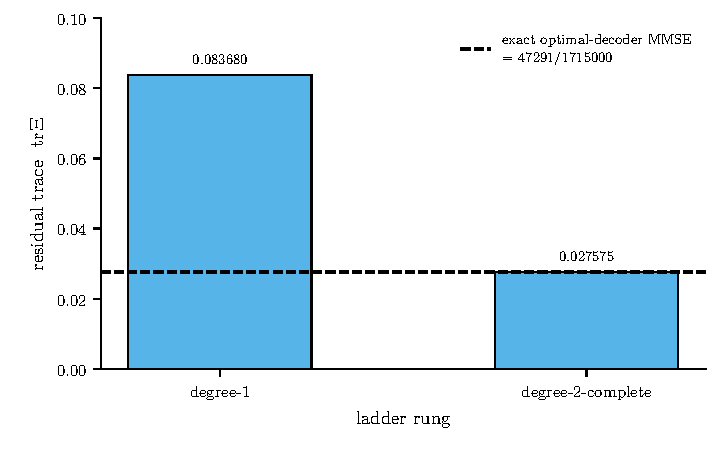
\includegraphics{figures/generated/fig_F4_e3_degree_ladder.pdf}
\caption{Degree-ladder contraction on REP(3) under N1 (E3). The degree-2-complete rung's residual equals the enumerated optimal-decoder MMSE exactly: both are $47291/1715000$, and the recorded difference is exactly $0.0$ (\gExact). The complete degree-2 family generates every function of the REP(3) syndrome, so its linear-estimator floor \emph{is} the true optimal-decoder MMSE, not an approximation to it.}% F-046, F-010 (C-10)
\label{fig:ladder}
\end{figure}

\paragraph{Selection beats baselines at every budget.} On SURF(3), greedy chain-rule check selection contracts the residual from the no-check baseline $0.4345$ to the full-schedule $0.1754$, and at \emph{every} intermediate budget its residual is at or below every tested baseline (lexicographic order and 10 seeded random orders; Figure~\ref{fig:budget}; \gRegPos). % F-044, F-045, F-009 (C-11)
This is a registered comparison against the tested baselines, not a general optimality statement: only the first greedy step is optimal by construction. Greedy selection carries the classical $(1-1/e)$ guarantee only for submodular objectives~\cite{nemhauser1978greedy,krause2008sensor}, and variance reduction by a set of regressors is not submodular in general~\cite{das2011submodular}, so no such guarantee is claimed here. The greedy selector also stops before exhausting a duplicate-padded candidate list rather than spending budget on provably worthless checks (\gRegPos). % F-012

\begin{figure}[htbp]
\centering
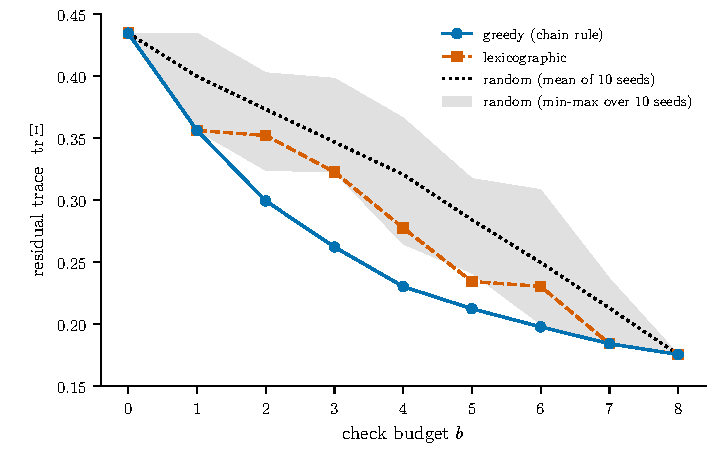
\includegraphics{figures/generated/fig_F3_e3_coverage_vs_budget.pdf}
\caption{Residual trace versus check budget under chain-rule greedy selection on SURF(3) (E3). Greedy is at or below the lexicographic order and every one of 10 seeded random orders at every budget (\gRegPos). This is a comparison against the tested baselines, not a general optimality statement: only the $b = 1$ step is optimal by construction.}% F-044, F-045, F-009 (C-11)
\label{fig:budget}
\end{figure}

\subsection{Existence: the certificate does classification work (E4)}
\label{sec:results-existence}

The typed existence certificate was computed on ground-truth Markov cycle models (\gExact{} for the REP rows). The baseline package---REP(3), N1 noise, the standard decoder---certifies: $\delta = 0.007144875$, $\varepsilon = 0.00725$ (the theorem bound $\delta \le \varepsilon$ visibly tight), multiplicity 2, status \texttt{certified}. % F-048 (C-13)
The deliberately broken decoder (mapping everything to one logical state) is caught by the multiplicity guard: $\delta = 0$ \emph{exactly}---perfect idempotence---but multiplicity 1 and status \texttt{trivialized} (\gRegPos{} for the guard). % F-049, F-016 (C-13, C-14)
This pair is the certificate idea in one contrast: a small idempotence defect alone would have certified the broken decoder; the typed certificate refuses. Sweeping the physical error rate under the sweep's defect-only rule (status \texttt{degrading} once $\delta$ exceeds $0.05$) flips the label from \texttt{certified} to \texttt{degrading} at $p = 1/5$ ($\delta$ rising monotonically $0.000298 \to 0.007145 \to 0.026432 \to 0.082368$ across $p \in \{1/100, 1/20, 1/10, 1/5\}$; \gExact). % F-050 (C-13)
At $p = 1/5$ the full typed classifier would return \texttt{trivialized} rather than \texttt{degrading}: no prototype remains stable there (multiplicity $0$, $\varepsilon = 0.104$), and multiplicity takes priority over the defect threshold (\gExact). % F-166 (C-13)
Table~\ref{tab:certificate} collects the classification.

\begin{table}[htbp]
\centering\footnotesize\setlength{\tabcolsep}{4pt}
\begin{tabular}{l r r r l}
\toprule
package & $\delta$ & $\varepsilon$ & mult. & status \\
\midrule
REP(3) + N1, standard decoder, $p = 1/20$ & 0.007144875 & 0.00725 & 2 & \texttt{certified} \\ % F-048
same, deliberately broken decoder & 0 (exact) & 0 & 1 & \texttt{trivialized} \\ % F-049
same, $p = 1/5$ (sweep rule) & 0.082368 & 0.104 & 0 & \texttt{degrading}$^{\dagger}$ \\ % F-050, F-166
\bottomrule
\end{tabular}
\caption{The existence certificate doing classification work on ground truth (\gExact). The broken decoder has \emph{perfect} idempotence---the multiplicity guard, not the defect, is what catches it. The remaining status, \texttt{non\_closed}, is thresholded on the closure deficit; its registered demonstration on the hidden-mode model was a \gRegNeg{} discussed in Appendix~\ref{app:predictions} (P4.2: the zero-deficit clause holds on the syndrome lens, not the frozen decoded lens). $^{\dagger}$The sweep assigns its label from the defect threshold alone; with multiplicity $0$ the full classifier would return \texttt{trivialized} at $p = 1/5$.} % F-048, F-049, F-050, F-014
\label{tab:certificate}
\end{table}

Two further certificate components behaved as designed on hidden-state models. The closure deficit correlates with an out-of-sample predictive gap across the model/horizon grid: Pearson $r = 0.936$ with the latching model N5 included (\gMeasured). % F-054 (C-15)
The registered bar $r \ge 0.9$ held (\gRegPos). % F-017 (C-15)
The same computation without N5 gives $r = -0.171$, which we report alongside; restricted to that narrow slice the registered correlation does not hold. % F-054 (C-15)
And the route-mismatch diagnostic exhibits the intended leakage signature on N5---a decoder lens that remains channel-accurate ($0.75$) while $RM$ grows severalfold over horizon (peak ratio $7.28\times$ baseline)---though it saturates below the frozen $10\times$ bar, a \gRegNeg{} discussed in Section~\ref{sec:negatives}. % F-052 (P4.3)

\subsection{Memory: exact witnesses, a genuine payoff, and a control that fired on us (E5)}
\label{sec:results-memory}

\paragraph{Witnesses separate the family exactly.} On the memoryless package (N1), the predictive-quotient audit finds \emph{zero} memory witnesses ($|Q| = |M| = 4$, $\Delta^{\max} = 0$; \gExact). On the hidden-mode package (N4) it finds 4 witnesses, MaxFiber 2, and an exact worst-case predictive gap $\Delta^{\max} = 112329952/1318359375 \approx 0.0852$; on the latching package (N5), 4 witnesses with $\Delta^{\max} = 539/1250 = 0.4312$ (\gExact). % F-028, F-029, F-030 (C-16)
These are certificates in the strict sense: exact rational statements that, within the declared catalog of histories, events, and continuations, currently indistinguishable histories assign different probabilities to some declared future event on N4/N5---by at most $\Delta^{\max}$---and identical probabilities on N1. Whether a decoder can turn that difference into performance is the separate, measured question below.

\paragraph{Currentization names the hidden coordinate.} Adding the mode bit as an observable dissolves the predictive surplus at candidate-set cardinality 1; no set of pure check bits does (\gRegPos). % F-021 (C-17)
The audit does not merely detect hidden memory---it identifies \emph{which} added observable would expose it.

\paragraph{The protocol trap fired against our hypothesis.} We built a two-phase alternating noise schedule as the intended ``schedule artifact,'' registering the prediction that internalizing the schedule (adding the phase as an autonomous state coordinate) would dissolve its witnesses, classifying it \texttt{artifact\_trap}. That prediction \emph{failed} as registered: internalization preserved all 4 witnesses and the package classifies \texttt{genuine\_memory\_after\_internalization} (\gExact{} for the classification). % F-032, F-070 (C-20)
The registered artifact hypothesis therefore failed (\gRegNeg). % F-020 (C-20)
The reading (\gInterp): a deterministic $p_0$-vs-$3p_0$ alternation carries real predictive content---the current phase predicts next-round statistics---so the trap correctly declined to call it an artifact. We state this carefully because it is easy to misreport: the control mechanism worked, and what it falsified was \emph{our} registered ``this is an artifact'' hypothesis. This is a negative result for that hypothesis, not a demonstration of the trap catching an artifact. % C-20

\paragraph{Memory's measured value, under a proper scoring rule.} The frozen accuracy-based payoff comparison came back nil, for a reason the diagnosis identified exactly: under X-only noise at $p < 1/2$, mode-conditional MAP correction picks the same coset representative in every mode, so accuracy-scored decoders tie by construction. A post-registration study (separately labeled, leaving all frozen verdicts untouched) rescored predictors on next-round negative log-likelihood, a strictly proper scoring rule~\cite{gneiting2007proper} (Figure~\ref{fig:payoff}), where memory has room to show non-tautological value. Findings (\gMeasured): the exact Bayes filter~\cite{rabiner1989hmm}, which reads the full round outcome (both syndrome bits and the logical increment), captures $0.00196$ of the $0.01061$ nats/round oracle ceiling at the frozen defaults and $0.03615$ of $0.05834$ at a declared louder operating point. % F-034, F-037 (C-18)
We read these as about 18\% and 62\% of ceiling (\gInterp). % F-040
A \emph{declared 2-state} run-length machine---driven by a two-bit slice of the outcome record (one syndrome bit and the logical increment), trained on the first half of each trajectory and scored on the second---captures a positive share ($0.00015$ and $0.00429$ nats/round), rising with machine size $K$ at the frozen defaults and up to $K{=}8$ in loud mode, where $K{=}16$ sits slightly below $K{=}8$ ($0.01036$ vs.\ $0.01052$; \gMeasured). % F-035, F-038 (C-18)
Naive per-step rounding of the continuous belief coordinate is \emph{value-destroying} below a resolution threshold: negative at every tested resolution at the frozen defaults (and non-monotone there, worst at $K{=}4$: $-0.0047$, $-0.0062$, $-0.0053$, $-0.0037$ for $K = 2, 4, 8, 16$), and negative in loud mode except at $K{=}16$, where a positive $+0.0301$ contradicted our pre-stated all-negative expectation and is reported as such (\gMeasured). % F-036, F-039 (C-19)
The packaging-theoretic reading (\gInterp): summarizing a short run-length statistic of the outcome record is cheap and safe; quantizing an \emph{internal belief} has a resolution threshold below which it destroys value. The run-length and rounding gaps are scored on different windows (second half vs.\ full trajectory), so their magnitudes are compared only qualitatively.

\begin{figure}[htbp]
\centering
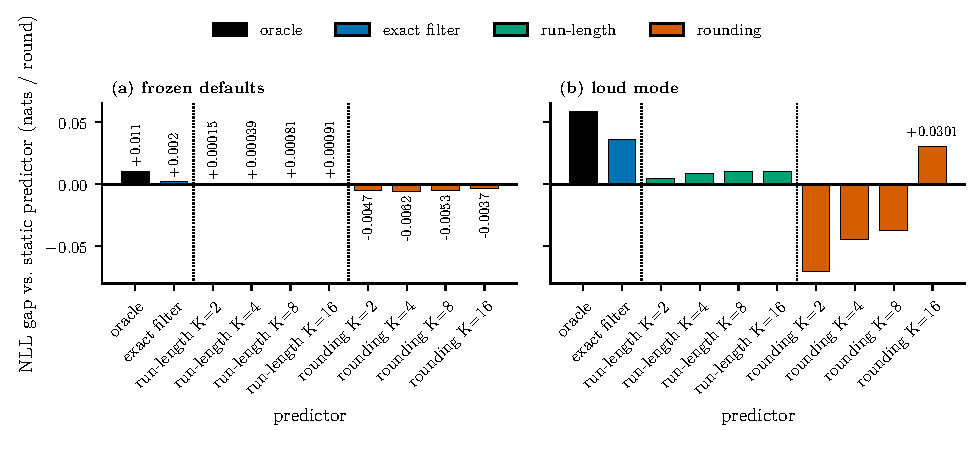
\includegraphics{figures/generated/fig_F5_e5_payoff_ladder.pdf}
\caption{Decoder-memory value under a proper scoring rule: next-round NLL gap over the static predictor on REP(3)+N4, at the frozen defaults (a) and the declared louder operating point (b) (E5, post-registration study; \gMeasured). The oracle is a ceiling, not deployable; the exact Bayes filter, which reads the full round outcome, is the realistic upper bound; run-length machines (driven by one syndrome bit and the logical increment, and scored on the second half of each trajectory while the other predictors are scored on the full trajectory) are positive and generally improve with $K$, with a slight loud-mode decline from $K{=}8$ to $K{=}16$; belief-rounding machines are value-destroying except the loud-mode $K{=}16$ point at $+0.0301$, a measured result reported as it stands, not an error bar. Values are printed beside the frozen-default bars, which are too small to read on the shared scale.}% F-034, F-035, F-036, F-037, F-038, F-039 (C-18, C-19)
\label{fig:payoff}
\end{figure}

\subsection{Pricing: exact machinery, negative evidence (E6)}
\label{sec:results-pricing}

The pricing audit is this paper's clean full negative, and we present it with the same prominence as the positives. The machinery itself is exact where declared and runs correctly: the exact value curve $V(b)$ by enumeration and the shadow-price curve $\lambda(b)$ (\gExact). % F-055, F-057 (C-21a)
The greedy selector's gap to the exact curve is at most $0.00405$ on REP(5) (\gMeasured). % F-056 (C-21a)
Every registered \emph{prediction} about pricing behavior failed at the frozen tolerances (\gRegNeg{} throughout): % C-21b
$\lambda$ was predicted nonincreasing after its maximum, and mixed degree-1/degree-2 costs instead produce sawtooth marginal values at budget parities; % F-022, F-071
a slack point $b^{*} < b_{\max}$ was predicted, and instead $b^{*} = b_{\max}$ for both code families because the frozen tolerance sits below the smallest genuine marginal value; % F-023, F-072
the consequence test (removing the last pre-slack unit should shift the sampled logical error rate detectably) did not separate: $\Delta = -0.000135$ against a combined standard error of $0.000119$; % F-059, F-073
and permuted proxy costs were strictly worse at only 36.9\% of budget points against a registered 80\% bar. % F-060, F-074
We do not soften this: as instantiated and thresholded here, the pricing primitive produced no positively evidenced result. The readings in Section~\ref{sec:negatives} suggest the failures are threshold-scale and test-design errors rather than refutations of the pricing concept (\gInterp), but on this prototype's evidence the primitive stands negative.

% ===========================================================================

\section{Results II: negative results as a taxonomy}
\label{sec:negatives}

Fourteen of the original build's 25 registered predictions failed as frozen. % F-147, F-148 (C-22)
Appendix~\ref{app:predictions} lists every one with its verdict and artifact; the frozen bars are in the public design documents and the measured values in each artifact's results file; none required changing any frozen parameter to diagnose. Here we do two things: classify the failures, and work one example of each class in enough detail that the reader can judge whether the diagnostic readings are honest. The classification (\gInterp): % C-23

\begin{enumerate}
\item \textbf{Bounds written at the wrong scale.} The prediction constrained the right quantity, but its bar was set at the scale of a different one.
\item \textbf{Thresholds frozen too strictly.} The predicted effect exists and points the right way, but the frozen numeric bar was set beyond what the effect delivers.
\item \textbf{Structure the prediction mischaracterized.} The measurement is informative and the machinery correct, but the world disagreed with the registered hypothesis.
\end{enumerate}

\paragraph{Worked example, class 1 (P1.1).} We registered that the full-schedule residual trace would fall below $10^{-2}$ at $p = 1/20$ and shrink $10\times$ from distance 3 to 5. Measured: $0.0837$ and $0.0740$, a ratio of $1.13$. % F-061, F-106
The bound was written at logical-error-probability scale, but $\operatorname{tr}\Xi$ is the linear-estimator MMSE of a $\pm1$ observable---a different quantity with a different scale and different distance behavior. The failure is real and taught us something concrete: the residual's units are variance of an observable, not failure probability, and predictions must be written in the object's own units. The linear-class limitation the number reflects is independently visible error-by-error: an exact bounded-weight cross-check shows that the affine estimator $A^{*}$ built from REP(5)'s four syndrome bits reproduces majority-logic minimum-weight decoding on 14 of 16 low-weight errors and fails on two (\gExact). That the failure is a limitation of the whole linear class, not of this one estimator, is our reading (\gInterp). % F-043

\paragraph{Worked example, class 2 (P6.2).} We registered that a slack point exists strictly before budget exhaustion, at tolerance $\lambda_{\mathrm{tol}} = 10^{-9}$. Measured: $b^{*} = b_{\max}$ for both REP(5) and SURF(3), because even the smallest genuine marginal value in these families exceeds the frozen tolerance. % F-072, F-058
The value curve itself is exact and its tail marginals are tiny (of order $10^{-5}$ to $10^{-4}$), % F-057
so the intended phenomenon---most of the budget buys almost nothing---is visibly present in the curve; the certificate failed because its threshold was frozen four to five orders of magnitude below the phenomenon. % F-057, F-058
A defensible re-thresholding would pass, and we did not do it, because a moved threshold after seeing data is exactly what the discipline forbids.

\paragraph{Worked example, class 3 (P5.3).} The protocol-trap prediction of Section~\ref{sec:results-memory}: we registered that our alternating schedule was an artifact that internalization would dissolve. Internalization preserved all 4 witnesses; the schedule carries genuine predictive content. % F-070
The machinery did precisely its job---it is the registered hypothesis that was wrong, and the failure sharpened the concept: ``externally scheduled'' does not imply ``predictively empty.'' For this package and its declared observation catalog, internalizing the schedule left every witness intact: the phase carried information about future observables, so the trap did not classify it as an artifact.

One more failure deserves mention here because the entire second half of the paper grows out of it: P2.1, the deployable drift witness that never detected within the tested grid (class 3, with an implementation-defect component). Its diagnosis and repair are Section~\ref{sec:arc}.

% ===========================================================================

\section{Results III: a registered failure, diagnosed and repaired inside the framework}
\label{sec:arc}

This section is the paper's centerpiece, and Figure~\ref{fig:cycle} is its map: a registered failure (E2), a diagnosis using the framework's own exact-input machinery, a corrected statistic re-registered with a \emph{predicted failure to beat the baseline} among its frozen predictions (E7), and two generalizations---to circuit-level noise (E8) and to closed-loop decoder control (E9). Throughout, E2's committed verdicts stand untouched; everything here is additive.

\begin{figure}[htbp]
\centering
\begin{tikzpicture}[
  x=1in, y=1in, font=\small,
  stage/.style={rounded corners=3pt, line width=0.6pt,
    align=center, inner sep=4pt, outer sep=0pt, minimum height=1.70in},
  substage/.style={rounded corners=3pt, line width=0.6pt,
    draw=black!50, fill=black!4, font=\footnotesize,
    align=center, inner sep=3pt, outer sep=0pt, text width=1.52in},
  flow/.style={-{Stealth[length=5pt,width=5pt]}, line width=0.8pt}
]
% A 6.5in by 4.6in canvas includes the legend and balanced outer margins.
\path[use as bounding box] (0,0) rectangle (\linewidth,4.60in);

% Top row: equal-height boxes and two 0.45in horizontal connectors.
\node[stage, draw=red!60!black, fill=red!8,
  text width=\dimexpr1.80in-8pt\relax] (s1) at (1.00,3.65)
  {E2: registered prediction P2.1 fails as frozen};
\node[stage, draw=blue!60!black, fill=blue!8,
  text width=\dimexpr1.85in-8pt\relax] (s2) at (3.275,3.65)
  {Exact-input diagnosis with the framework's own machinery: Walsh--Hadamard pmf inversion, $A^{*}$-lift energy compression, mis-scaled null};
\node[stage, draw=blue!60!black, fill=blue!8,
  text width=\dimexpr1.75in-8pt\relax] (s3) at (5.525,3.65)
  {Corrected statistic re-registered, including a prediction that the original scenario will \textsc{still} not beat the baseline};

% Bottom-left stage: one container with a heading and two internal boxes.
\node[stage, draw=black!50, fill=black!4, minimum width=1.80in]
  (s5) at (1.00,1.25) {};
\node[font=\small\bfseries, inner sep=0pt] at (1.00,1.92)
  {Generalization};
\node[substage, minimum height=0.68in] (e8) at (1.00,1.45)
  {E8: circuit level (Stim, $d{=}3$); $2\times$ bar met at the grid's thinnest margin};
\node[substage, minimum height=0.53in] (e9) at (1.00,0.775)
  {E9: closed recalibration loop on a known drifting channel};

% Bottom-right stage: one rounded outline, equal halves, one divider.
\begin{scope}
  \clip[rounded corners=3pt] (2.35,0.40) rectangle (6.40,2.10);
  \fill[green!10] (2.35,0.40) rectangle (4.375,2.10);
  \fill[orange!12] (4.375,0.40) rectangle (6.40,2.10);
\end{scope}
\draw[green!50!black, line width=0.6pt, rounded corners=3pt]
  (4.375,0.40) -- (2.35,0.40) -- (2.35,2.10) -- (4.375,2.10);
\draw[orange!70!black, line width=0.6pt, rounded corners=3pt]
  (4.375,2.10) -- (6.40,2.10) -- (6.40,0.40) -- (4.375,0.40);
\draw[black!50, line width=0.6pt] (4.375,0.40) -- (4.375,2.10);
\node[align=center, inner sep=4pt,
  text width=\dimexpr2.025in-8pt\relax] at (3.3625,1.25)
  {E7 off-support $(4,8)$: W2b at full detection by $N{=}1000$; neither baseline meets the criterion within the grid};
\node[align=center, inner sep=4pt,
  text width=\dimexpr2.025in-8pt\relax] at (5.3875,1.25)
  {E7 original $(0,3)$: predicted failure to beat the baseline held (baseline 1000 vs.\ corrected 4000)};
\coordinate (s4north) at (5.525,2.10);
\coordinate (s4west) at (2.35,1.25);

% The only arrows are the five straight edges of the clockwise loop.
\draw[flow] (s1.east) -- (s2.west);
\draw[flow] (s2.east) -- (s3.west);
\draw[flow] (s3.south) -- (s4north);
\draw[flow] (s4west) -- (s5.east);
\draw[flow, line width=1.4pt] (s5.north) -- (s1.south);

\node[font=\small, align=center, text width=3.10in, inner sep=0pt]
  (thesis) at (3.25,2.45)
  {\textbf{the framework audits and repairs\\its own instrument}};

\node[font=\footnotesize, align=center, text width=6.30in, inner sep=0pt]
  at (3.25,0.175)
  {red = registered failure; blue = framework-internal diagnosis and re-registration; green = registered positive; amber = predicted negative that held};
\end{tikzpicture}

\caption{The diagnosis-and-repair cycle of this section. A registered failure (E2, red) is diagnosed with the framework's own exact-input machinery (blue); the corrected statistic is re-registered together with a prediction that the original scenario will \emph{still} not beat the baseline (blue); the predicted negative holds while the off-support scenario detects (amber / green); and the correction generalizes to circuit level (E8) and to a closed loop (E9). The label inside the loop states the arc's thesis: the framework audits and repairs its own instrument.}% C-03
\label{fig:cycle}
\end{figure}

\subsection{The failure (E2)}
\label{sec:e2}

E2 tested drift detection on SURF(3): declared model N2 ($p = 3/100$), true model N3 (the same plus an unmodeled correlated $ZZ$ injection, $q = 1/50$, on the frozen qubit pair $(0,3)$). Two witnesses were tested against a matched decoder-failure-rate baseline: W1, an \emph{oracle} witness with simulator access to true logical values (labeled non-deployable from the start), and W2, the deployable-shaped, syndrome-only witness---the one that would matter in practice. Results (\gMeasured): W1 detected at $N = 500$ shots vs.\ the baseline's $1000$---a real $2\times$ improvement, short of the registered $4\times$ bar---and W2 \emph{never detected within the frozen grid} (up to $N = 16000$). Both registered predictions failed (\gRegNeg). % F-026, F-005 (C-24)
Null calibration passed: false-positive rates 0.0 (W1) and 0.02 (W2) at the frozen bar. % F-027

\subsection{The diagnosis: exact inputs, and mostly about the test itself}
\label{sec:diagnosis}

Before any correction code was written, the failure was analyzed with the same moment engine the audits are built on: the mean shifts, covariance blocks, and syndrome distributions below are exact rational objects, and the scalar energies and divergences reported from them are floating-point evaluations of those exact inputs. The four findings were then pinned as tests in the repository, so they are commitments, not narrative. The reflexive point we draw from findings 1 and 2 is an analogy, marked as such (\gInterp): the same moment machinery that audits a schedule's coverage of the logicals was turned on the witness itself, to ask how much of the drift signal it kept.

\paragraph{Finding 1: the statistic discards its mean signal (\gExact).} W2 was built from \emph{centered} covariance blocks, so the drift's direct first-moment signal entered it only through its second-order footprint, never as a mean feature. The frozen injection's exact mean shift is zero on seven of eight native checks and $-331776/9765625 \approx -0.0340$ on the eighth, with total energy $\|\Delta\mathrm{mean}_L\|^{2} = 0.0011542$, a floating-point sum of the exact entries. % F-075 (C-25)
A real, exactly quantified direct signal was being left out of the feature set.

\paragraph{Finding 2: the lift built for the wrong objective compresses the signal $\approx 73\times$.} W2 lifted the syndrome-covariance defect through the coverage-optimal map $A^{*}$---a map fit to predict \emph{logical values}, not to preserve \emph{drift sensitivity}. The drift signal's energy before the lift is $\|\Delta K_{LL}\|_F^{2} = 0.0032632$; after, $4.4703 \times 10^{-5}$ (floating-point norms of exact covariance differences). % F-076 (C-26)
The compression ratio $\approx 73\times$ is our reading of those two numbers (\gInterp).

\paragraph{Finding 3: a borrowed null (\gInterp, confirmed by measurement below).} W2's alarm threshold was calibrated on W1's statistic---a differently scaled object---rather than on W2's own null distribution. % F-077 (C-27)

\paragraph{Finding 4: the frozen scenario is structurally hard for \emph{any} syndrome-only method.} The key move: because means of XOR-combinations of checks are Walsh--Hadamard coefficients of the syndrome distribution (Section~\ref{sec:domain}), the full $2^{8}$-outcome native-check syndrome pmf is \emph{exactly} recoverable under both the declared and true models, hence so is the syndrome distribution under both models (\gExact). From those exact distributions, the per-shot Kullback--Leibler divergence $D(\mathrm{true}\,\|\,\mathrm{declared})$ of the syndrome channel, in nats per shot, is evaluated numerically; by Stein's lemma it is the exponential rate at which i.i.d.\ samples discriminate the two hypotheses~\cite{cover2006elements}. We compare it with the per-shot divergence of the logical-failure channel, measured from $N = 2 \times 10^{6}$ shots per scenario (\gMeasured), over three injection pairs: % F-078 (C-28a, C-28b)

\begin{table}[htbp]
\centering\footnotesize
\setlength{\tabcolsep}{3.5pt}
\begin{tabular}{l l r r r}
\toprule
Pair & Relation to logical support & syndrome KL/shot & failure KL/shot & ratio \\
 & & (from exact pmf) & (measured) & \\
\midrule
$(0,3)$, the frozen E2 pair & 2 of 3 qubits of $\bar{Z}$ & 0.006151 & 0.009247 & 0.665 \\ % F-078
$(2,5)$ & 1 qubit touches $\bar{X}$ & 0.010823 & 0.009841 & 1.100 \\ % F-078
$(4,8)$ & off both logical supports & 0.051352 & 0.000066 & 773.4 \\ % F-078
\bottomrule
\end{tabular}
\caption{Per-shot KL divergence (nats/shot) available to the syndrome channel, evaluated from the exactly recovered pmf, vs.\ the logical-failure channel, measured; the ratio is therefore a measured quantity (\gMeasured). The frozen E2 pair $(0,3)$ sits, by construction, nearly on a minimum-weight logical-failure path: the failure channel carries more per-shot information about such drift than the syndrome does (ratio $< 1$), while for the off-support pair the syndrome channel carries $\approx 773\times$ more. Per-shot divergence is a discrimination rate, not a finite-sample latency ratio.} % F-078 (C-28a, C-28b)
\label{tab:kl}
\end{table}

The structural reading (\gInterp): drift that feeds a minimum-weight failure path is exactly the drift the failure channel is built to notice and the syndrome channel is built to correct silently. Among the three scenarios, the E2 pair is the one that puts a syndrome-only witness at the greatest disadvantage relative to failure-rate monitoring---a fact about this scenario grid, not a general worst-case statement---independent of, and in addition to, findings 1--3. This finding drove the design of the re-registration: the corrected witness had to be tested across the \emph{range} finding 4 exposes, with an honest prediction attached to each regime.

\subsection{The corrected witness, re-registered---including a predicted failure (E7)}
\label{sec:e7}

The correction unifies findings 1 and 2 in one object: the vector of means of the degree-$\le 2$ probe family (all 8 native checks plus all 28 pairwise XOR products---36 exact Walsh--Hadamard coefficients), used \emph{directly}, with no centering and no lift. The corrected detection statistic is the whitened quadratic form (a model-referenced Mahalanobis form of Hotelling type~\cite{hotelling1931ratio}; unlike the classical $T^{2}$, the covariance is the declared model's, not a sample estimate)
\begin{equation}
T \;=\; (\hat\theta - \theta_{\mathrm{model}})^{\top}\, \Sigma_{\theta}^{+}\, (\hat\theta - \theta_{\mathrm{model}}),
\label{eq:w2b}
\end{equation}
with $\theta_{\mathrm{model}}$ and the estimator covariance $\Sigma_\theta$ exact under the declared model and the threshold calibrated on the statistic's own null by seeded parametric bootstrap (Monte Carlo draws from the declared model)~\cite{efron1979bootstrap}. Around it, a ladder of four rungs was registered: the \emph{old} statistic with its null merely recalibrated (isolating finding 3); the quadratic statistic of Eq.~\eqref{eq:w2b}; a matched-filter \emph{naming} step (a dictionary of nine exact per-qubit drift signatures, whitened, inner-product-matched, then forward-mapped to a logical direction); and a CUSUM sequential wrapper~\cite{page1954continuous}---with the baseline given the \emph{same} sequential upgrade, which removes one test-design asymmetry between the two sides (it does not equalize their operating characteristics; the null-rate checks below report those separately). Seven predictions were frozen from finding 4's numbers before implementation. Three outcomes carry the section (Figure~\ref{fig:e7}):

\paragraph{The off-support scenario: a dramatic, registered win.} On pair $(4,8)$---where Table~\ref{tab:kl}'s measured ratio put $\approx 773\times$ more per-shot information in the syndrome channel---the corrected rungs detect at $N = 1000$ (quadratic and naming rungs) and $N = 2000$ (sequential), while neither baseline reaches the detection criterion ($\ge 9/10$ seeds) anywhere in the frozen grid up to $N = 16000$ (\gRegPos{} against a conservative registered $10\times$ bar). % F-078, F-080 (C-28b, C-30)

\paragraph{The original scenario: the predicted failure held.} We registered, in advance, backed by Table~\ref{tab:kl}'s ratio of $0.665$, that on the original E2 pair $(0,3)$ \emph{no corrected rung would beat the baseline}. That is what happened: baseline $N = 1000$; best corrected rungs $N = 4000$ (\gRegPos---a predicted negative that held). % F-081 (C-31)
We give this result more narrative weight than the win above, deliberately. A correction developed after a failure invites the suspicion of post-hoc storytelling---of a statistic quietly tuned until the old test passes, the degenerating move in Lakatos's sense~\cite{lakatos1978methodology}. A frozen, exact-computation-backed prediction that the correction would \emph{still lose} on the original test, which then held, is the strongest evidence this arc can offer that the diagnosis was explanatory rather than curve-fitting. The near-parity scenario $(2,5)$, registered as descriptive with no bar, landed where its ratio of $1.100$ suggested: baseline $1000$; quadratic and naming rungs $2000$; sequential rung $8000$ (\gMeasured). % F-082

\paragraph{The honest residue.} Three E7 predictions failed (\gRegNeg{} each). The recalibrated-null prediction P7.1 failed: we predicted the old statistic's own-null threshold would be $\le 10\%$ of the borrowed one, and measured a ratio of $1.33$. % F-079 (C-29)
The reading (\gInterp): our $O(p)$-vs-$O(p^2)$ reasoning had described the \emph{injected signal's} scale, not the \emph{null-fluctuation} scale a threshold actually calibrates.
Naming split (Figure~\ref{fig:naming}): only 3/10 detecting seeds named a qubit in the true injection pair (bar: 8/10), while the forward-mapped logical-direction overlap was $0.869$, above its $0.6$ bar (\gMeasured). % F-083 (C-32)
The reading (\gInterp): the overlap is taken in the two-dimensional space of the selected logical observables, onto which the nine per-qubit drift signatures map to few distinct directions, so direction overlap is a coarse check that detection and direction-naming can pass while qubit-level naming stays hard. The headline quadratic rung W2b's null false-positive rate came in at 6\% against the 2\% bar (all other rungs passed). % F-084 (C-32)

\begin{figure}[htbp]
\centering
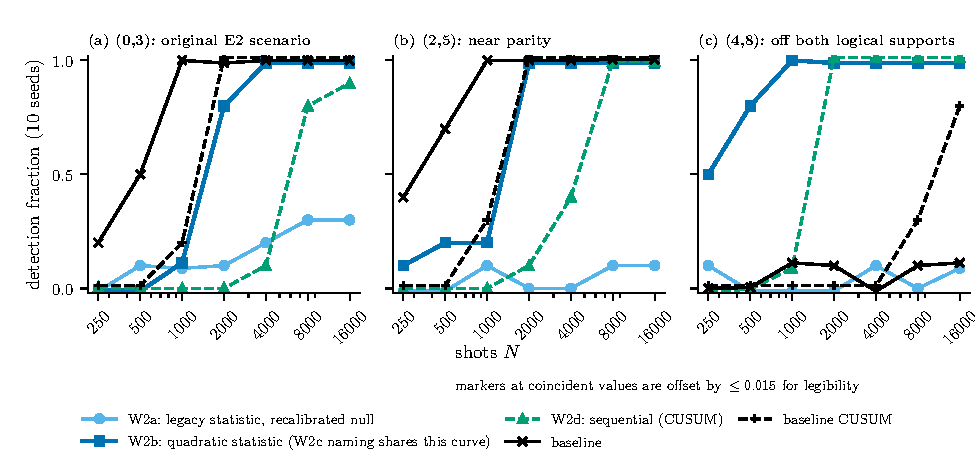
\includegraphics{figures/generated/fig_F6_e7_detection_ladder.pdf}
\caption{Corrected-witness detection fraction versus shots across the E7 scenario grid, 10 seeds per point (\gMeasured). (a) The original E2 pair $(0,3)$: the baseline detects first, which was the registered, expected outcome, not a surprise (P7.3; \gRegPos{} as a predicted negative that held). (b) The near-parity pair $(2,5)$, registered as descriptive with no bar. (c) The off-support pair $(4,8)$: the quadratic statistic W2b (whose detection curve the naming rung W2c shares) reaches full detection at $N = 1000$ while neither baseline reaches the $\ge 9/10$ detection criterion anywhere in the grid; W2a is the legacy statistic with only its null recalibrated (\gRegPos{} against a registered $10\times$ bar).}% F-080, F-081, F-082 (C-30, C-31)
\label{fig:e7}
\end{figure}

\begin{figure}[htbp]
\centering
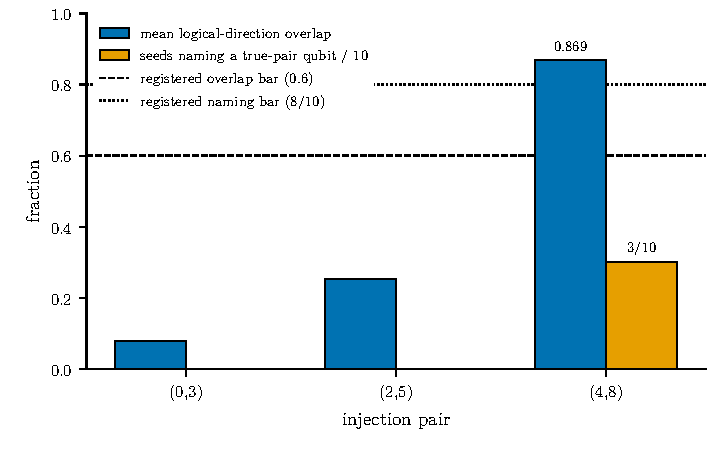
\includegraphics{figures/generated/fig_F7_e7_naming_overlap.pdf}
\caption{The E7 naming outcome (P7.5; \gRegNeg). On the off-support pair $(4,8)$ the forward-mapped logical-direction overlap is $0.869$, above the registered $0.6$ bar, while only 3 of 10 detecting seeds named a qubit in the true injection pair, below the $8/10$ bar. Pairs $(0,3)$ and $(2,5)$ are shown for context; the prediction concerned $(4,8)$. The reading (\gInterp): the overlap is taken in the two-dimensional space of the selected logical observables, onto which the nine per-qubit signatures map to few distinct directions, so it is a coarse check that cannot discriminate between qubits on its own.}% F-083 (C-32)
\label{fig:naming}
\end{figure}

\subsection{Generalization to circuit-level noise (E8)}
\label{sec:e8}

The corrected statistic generalizes directly to circuit level: detectors replace checks, the degree-$\le 2$ family becomes detectors plus pairwise XOR products (40 detectors, 820 features for the rotated $d{=}3$ Stim memory circuit used), % F-088
and---because the prototype has no exact moment engine at circuit level---$\theta_{\mathrm{model}}$ and $\Sigma_\theta$ are estimated from a large declared-model calibration sample ($2 \times 10^{5}$ shots), with predictions frozen from a disjoint-seed pilot before the scored run (Section~\ref{sec:methods-registration}). % F-089
The scored drift scenario is a global $2\times$ error-rate increase; the baseline is the PyMatching logical-failure rate under the same detection framing.

Result (Figure~\ref{fig:e8}): the witness detects at $N_{\mathrm{det}} = 50$ vs.\ the baseline's $100$, clearing the pilot-frozen $2\times$ bar exactly---which, on the discrete grid $\{10, 20, 50, 100, 250, 500, 1000, 2000\}$, is the thinnest margin the grid can resolve, and this result must be read with that caveat attached, not as a comfortable win (\gRegPos, margin caveat mandatory). % F-086 (C-33)
Null false-positive rates were 0\% for both sides (\gRegPos). % F-087
We report one more thing the deviations log preserves: the pilot had suggested $\approx 5\times$; the scored run delivered $2\times$. The pilot number is a smaller-sample estimate and is not the headline. % F-167, F-086

\begin{figure}[htbp]
\centering
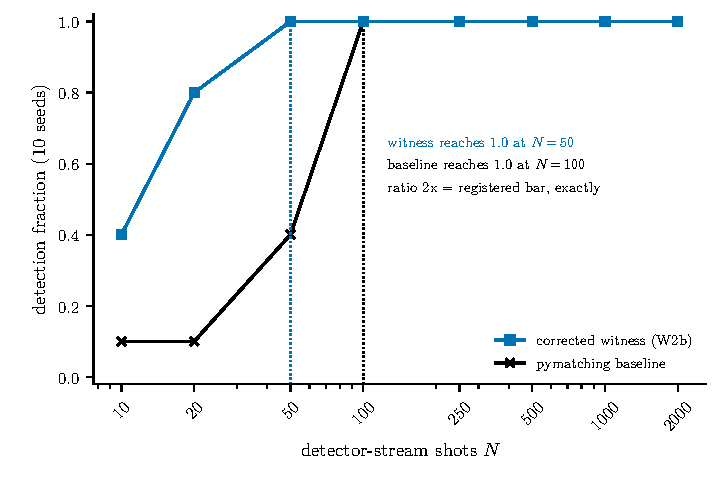
\includegraphics{figures/generated/fig_F8_e8_circuit_level.pdf}
\caption{Circuit-level detection fractions under a global $2\times$ rate drift on the rotated $d{=}3$ Stim memory circuit, 10 seeds (E8; \gRegPos). The corrected witness reaches full detection at $N_{\mathrm{det}} = 50$ and the PyMatching baseline at $100$: the witness clears the pilot-frozen $2\times$ bar exactly, at the thinnest margin this discrete grid can resolve, and not by a comfortable margin.}% F-086, F-088 (C-33)
\label{fig:e8}
\end{figure}

\subsection{Closing the loop: witness-triggered decoder recalibration (E9)}
\label{sec:e9}

The final experiment asks whether the witness's information is worth anything \emph{operationally}: does the witness's \emph{timing} buy logical fidelity per unit of recalibration budget, when the drifting channel is known by construction and only \emph{when} to recalibrate is at issue? On an epoch-discretized circuit-level timeline (72 detectors, 2628 degree-$\le 2$ features) % F-090
with a heterogeneous drift injected partway through (one measurement-flip channel elevated $20\times$---a uniform global rescale was verified, before freezing anything, to give minimum-weight matching nothing to recalibrate, and the scenario was corrected and logged), five decoder policies run over 10 seeds: \emph{static} (never recalibrate; floor), \emph{oracle} (switch to the true-model decoder at the true drift epoch, without charging a recalibration event; ceiling), \emph{budget-matched blind schedule}, \emph{high-budget blind schedule} ($\approx 5\times$ the events), and the \emph{witness-triggered} policy (recalibrate when the sequential witness fires, self-correcting on false alarms).

The budget matching deserves one sentence of methodology, because it is where an experiment like this is easiest to rig accidentally: the matched schedule was forced, per seed, to spend \emph{exactly} the same number of recalibration events the witness policy spent on that seed (realized counts $[1,1,2,2,1,1,3,2,1,2]$, identical lists for both policies; mean 1.6), % F-093
after the first frozen run was caught in internal review: its schedule had been set to a fixed period aimed at one event per run while the witness policy's realized mean was $1.6$, so the budgets were not matched even in aggregate. The schedule was corrected to exact per-seed matching and the implementation re-run and re-frozen, with the prediction bars unchanged (Appendix~\ref{app:deviations}).

Results (Figure~\ref{fig:e9}; post-drift logical error rate per epoch, mean over seeds; grade per item):
\begin{itemize}
\item Witness-triggered: $0.0930$, about $0.0014$ above the oracle ceiling's $0.0916$ (gap $0.00143$ to three significant figures; frozen bar: within $0.01$; \gRegPos). % F-091 (C-34; rounding authorized in claims.md)
\item Against the genuinely budget-matched blind schedule: $0.0930$ vs.\ $0.1115$---the witness wins by $0.0185$ at \emph{identical} per-seed budgets (\gRegPos). % F-092, F-093 (C-34)
\item The static floor sits at $0.1185$. % F-097
\item The high-budget schedule ($\approx 5\times$ the events) scores $0.0946$, and its $0.0016$ deficit to the witness policy is smaller than the $\approx 0.002$ estimated paired standard error at 10 seeds---statistically unresolved, and we state so in the same breath as the number (\gMeasured, no bar). % F-094, F-095 (C-35)
\item Pre-drift trigger rates, descriptive: witness 0.0 on the scored seeds; the schedules trigger by construction (0.5 and 1.0 of seeds recalibrating pre-drift at least once). % F-096
\end{itemize}

Two scope statements bound this result. First, the resolved claim is \emph{witness beats budget-matched blind scheduling}; whether it beats \emph{frequent} blind scheduling is unresolved at this sample size---spending $\approx 5\times$ the budget blindly closes most, not all, of the gap. % C-35
Second, E9's recalibration deliberately searches only the one channel known by construction to drift: it demonstrates the \emph{timing and budget} value of the witness, not drift \emph{identification}, which is E7's naming step, tested separately. % C-39 (F-105)

\begin{figure}[htbp]
\centering
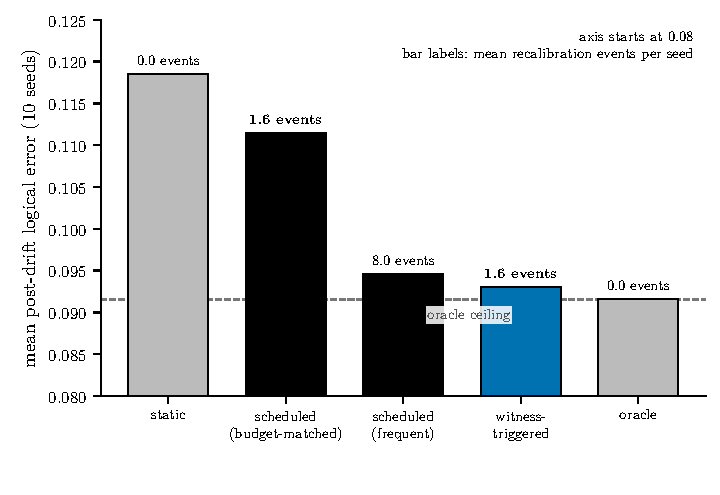
\includegraphics{figures/generated/fig_F9_e9_closed_loop.pdf}
\caption{Closed-loop decoder recalibration (E9): mean post-drift logical error per epoch over 10 seeds, with each policy's mean recalibration events per seed above its bar (\gMeasured). Recalibration here re-estimates the one channel known by construction to drift; the oracle switches to the true-model decoder at the drift epoch without spending a recalibration event, which is why it shows $0.0$ events. The witness-triggered policy and the budget-matched blind schedule spend identical realized event counts on every seed (counts between 1 and 3, mean $1.6$), and the witness wins by $0.0185$ (\gRegPos). The frequent schedule spends about $5\times$ the budget; its $0.0016$ deficit to the witness is smaller than the $\approx 0.002$ paired standard error at 10 seeds and is statistically unresolved, so this figure does not show that the witness beats frequent blind recalibration.}% F-091, F-092, F-093, F-094, F-095 (C-34, C-35)
\label{fig:e9}
\end{figure}

% ===========================================================================

\section{Related work}
\label{sec:related}

The QEC mechanics this paper touches are established, and we state the overlaps specifically rather than generically. Calibrating noise models from pairwise detector correlations---the $p_{ij}$ estimator and the edge-weight formula $w_{ij} = \log((1-p_{ij})/p_{ij})$---is standard experimental practice~\cite{fowler2014scalable,chen2021exponential}, deployed at scale in Google's surface-code experiments~\cite{google2023suppressing,acharya2025belowthreshold}; detector statistics have likewise been used to detect and remove correlated/leakage errors~\cite{mcewen2021removing}; E9's own recalibration is simpler than any of these: it matches the mean detector-flip rate to a simulated candidate curve for the one channel known to drift and rebuilds the decoder from that candidate's detector error model, and hidden-Markov inference on repeated syndrome records to detect leakage~\cite{bultink2020leakage,varbanov2020hmm}. Estimating the noise model from syndrome statistics alone, without disturbing the logical information, has its own literature: the in-situ estimation proposals of~\cite{fujiwara2014instantaneous,combes2014insitu}, identifiability results~\cite{wagner2021optimal,wagner2022paulichannels}, and detector-model and correlated-noise learning from experimental syndrome data~\cite{chen2022calibrated,harper2023correlated,gicev2024syndrome,remm2025syndromecorrelations,blumekohout2025dem}. Reweighting a matching decoder's graph in response to drifting noise is the direct subject of prior work~\cite{spitz2018adaptive,huo2017realtime,dgr2023reweighting}, and calibrating decoder priors to correlated or device-specific noise likewise~\cite{nickerson2019correlated,sivak2024priors}. Among the closest neighbors of Section~\ref{sec:arc}'s drift witness that our bounded literature search found are the time-varying syndrome estimators of~\cite{kobori2025bayesian,bhardwaj2025drifting} and the drift-triggered recalibration of~\cite{poster2026reloqate}; in-situ recalibration of physical controls during repeated error detection was demonstrated by~\cite{kelly2016insitucalibration}. Drift itself is a characterized phenomenon~\cite{proctor2020drift}. Trading measurement budget against decoding quality by measuring fewer or adaptively chosen checks is likewise established~\cite{berthusen2024partialsyndrome,tansuwannont2023adaptivesyndrome,berthusen2025adaptivesyndrome}, though not by a coverage-residual objective. Sequential change detection via CUSUM is classical~\cite{page1954continuous}. Our simulation and decoding infrastructure is Stim~\cite{gidney2021stim} and PyMatching~\cite{higgott2022pymatching,higgott2025sparseblossom}, used as documented libraries. Relative to all of this, the present work claims no mechanism novelty. What it adds is orthogonal: a certificate framing in which coverage, existence, memory, and price are typed audit objects derived from one framework; an exact-computation layer (the Walsh--Hadamard syndrome-pmf inversion driving Section~\ref{sec:diagnosis}) used, after E2 had failed, to \emph{explain} why a detector-statistic method failed, and then to predict in advance where its corrected form would and would not win; and a pre-registration discipline under which the framework's predictions---including predictions of its own failure---were frozen and scored.

On the SBT side, this paper consumes the corpus~\cite{sbt-f1,sbt-f3,sbt-xi,sbt-hol,sbt-pt,sbt-ng,sbt-cast,sbt-xor,sbt-spend,sbt-qm,sbt-hid,sbt-nk} as its specification and tests it; it does not extend the theory. The instantiated formulas are cited object-by-object in Appendix~\ref{app:formulas}, and Section~\ref{sec:sbt} notes, primitive by primitive, the established external concepts (lumpability, causal states, projection-operator memory) that the instantiated objects have as counterparts.

% ===========================================================================

\section{Discussion: what this does and does not establish}
\label{sec:discussion}

\paragraph{Established, on this prototype's evidence (our synthesis of the claim inventory; \gInterp).} Four SBT primitives, forced into a real technical domain, each produced a concrete, machine-checkable audit object whose behavior on ground truth matched its intended semantics: a coverage residual that lands exactly on the enumerated optimal MMSE where theory says it must; an existence certificate whose typed statuses do genuine classification work, including refusing a trivialized decoder; an exact memory witness with a quantified, rational worst-case gap and a currentization step that names the hidden coordinate; and a protocol-trap control that operated correctly against our own hypothesis. % C-01
The falsification discipline was real: 14 of 25 original predictions failed as frozen and none was tuned away. % F-148, C-02
And the discipline was \emph{productive}: the framework's exact-input machinery diagnosed one of its own registered failures, predicted in advance both where the corrected instrument would win and where it would keep losing, was right on both, and carried the correction to circuit level (clearing its bar at the thinnest margin the grid resolves) and to a closed control loop on a known drifting channel, with the unresolved frequent-schedule comparison stated. % C-03

\paragraph{Not established.} No hardware evidence of any kind; everything is classical simulation of small codes. % C-05
No claim that $\Xi \succ 0$ precludes a nonlinear decoder. % C-04
No claim that the corrected witness beats failure-rate monitoring in general---the advantage is scenario-dependent, and the original E2 scenario is our own registered counterexample. % C-31
No claim that witness-triggering beats \emph{frequent} blind recalibration (unresolved at this sample size); the resolved comparison is budget-matched. % C-35
No positive evidence for the pricing primitive, whose registered predictions all failed; % C-21b
and no evidence at all regarding transport/functoriality, which was never built. % C-01
No Born-rule, Bell, or coherent-dynamics claims, and no asymptotic-threshold claims: every result is finite-carrier classical simulation. % C-05
No fitted macro model is used as evidence; fitted quantities are diagnostic only. % C-05
No cross-audit inference: stability does not establish nontrivial storage, coverage and existence do not imply one another, and memory witnesses and drift do not imply one another. % design/04 §1
No drift-identification claim from E9: its recalibration acts on the one channel known by construction to drift, so it evidences the timing and budget value of the witness only. % C-39
Nothing here validates SBT's broader ambitions in other domains: one domain, honestly instrumented, is one data point.

\paragraph{What the exercise suggests about frameworks for emergence.} The pattern this prototype exhibits---primitives that compile to computable certificates, nulls that can fire against the theory's own favorite conclusions, predictions frozen before the scored runs, and a repair loop that runs \emph{inside} the framework---is, we think, the appropriate evidentiary standard for any theory of emergence that wants to be more than vocabulary. Quantitative accounts of emergence outside SBT likewise tie a macro-level description to a computable criterion: coarse-grained predictability~\cite{israeli2006coarse}, effective information~\cite{hoel2013causal}, dynamical independence~\cite{barnett2023dynamical}. That they share the falsifiability demand as well is our reading (\gInterp), not a claim those works make. Judged by that standard, four of SBT's six primitives produced positively evidenced objects here, one (pricing) returned a clean registered negative---which is the discipline working, not failing---and one abstained. Whether the framework's primitives continue to earn their keep is now an empirical question with a template: pick a domain with a packaging structure, instantiate, register, run, and report the failures at the same volume as the wins.

% ===========================================================================

\section{Reproducibility statement}
\label{sec:repro}

Everything reported above regenerates from the public repository. The known-good environment (exact versions all reported numbers were measured against): Python 3.10.12, numpy 2.2.6, scipy 1.15.3, stim 1.16.0, pymatching 2.4.0, matplotlib 3.10.8, pytest 9.0.2. % F-169
The dependency floors in \texttt{pyproject.toml} are lower bounds, not pins; to reproduce the exact environment, install those versions explicitly. % F-160, F-161
Setup and verification:

\begin{verbatim}
pip install -e ".[dev]"              # package + pytest
pytest -q                            # 170 tests pass
python -m sbqos.reproduce_all        # nine experiments; manifests verified
python -m sbqos.reproduce_all        # second run; compare byte-for-byte
python paper/figures/make_figures.py # figures F3-F9 (deterministic)
\end{verbatim}

The prototype's suite passes 149 tests (127 from the original build, 22 from the follow-up), and 21 further tests cover the paper's figure pipeline; % F-145, F-168
the theorem-anchoring tests are % F-162
\begin{itemize}[nosep]
\item \texttt{test\_thm\_chain\_rule\_rep5\_seeded\_splits\_exact},
\item \texttt{test\_thm\_top\_ladder\_rep3\_mmse\_matches\_bruteforce\_exact},
\item \texttt{test\_thm\_B5\_lumpable\_zero\_deficit\_for\_syndrome\_lens}.
\end{itemize}
Each \texttt{reproduce\_all} run regenerates the nine experiments and verifies its own freshly written manifest; the evidence recorded for this paper is stronger than that: two consecutive runs produced byte-identical files, and their nine manifest root hashes equal the ones recorded in the repository report (wall clock $\approx$ 13--14 minutes per run on the reference machine). % F-159, F-149..F-157
each experiment directory contains its frozen configuration, results, SHA-256 manifest, environment record, and every figure's exact data as CSV. The nine manifest root hashes are recorded in the repository report so a reader can verify they regenerated the same evidence, not merely similar evidence. % F-149..F-157

% ===========================================================================


\appendix
\section{Notation}
\label{app:notation}

Paper symbols and their meanings, grouped by primitive. The repository uses code-level names documented alongside each symbol in the project's notation file; the paper uses only the symbols below.

\begin{table}[H]
\centering\small
\begin{tabular}{l p{10.5cm}}
\toprule
Symbol & Meaning \\
\midrule
\multicolumn{2}{l}{\emph{Packaging (Section~\ref{sec:sbt})}} \\
$Z, P, f$ & carrier state set, one-step Markov kernel, lens (macro label map) \\
$\mu$ & a carrier distribution (the argument of the packaging operator) \\
$u_x$ & prototype distribution of macro label $x$ \\
$Q_f, U_f$ & marginalization through the lens; lift of a macro label to its prototype \\
$E_{\tau,f} = U_f \circ Q_f \circ P^{\tau}$ & packaging operator at horizon $\tau$ \\
$\pi$ & stationary law of $P$ (replaced by a declared finite-horizon weighting for absorbing models) \\
$\sigma_a$ & $\pm1$ observable of Pauli vector $a$: $\sigma_a(e) = (-1)^{\langle a, e\rangle}$ \\
$L, D$ & native (scheduled) and dissolving (logical) probe families \\
\multicolumn{2}{l}{\emph{Coverage audit}} \\
$K_{LL}, K_{DL}, K_{DD}$ & covariance blocks of scheduled-check / logical $\pm1$ observables \\
$\Xires$ & adequacy residual: logical covariance invisible to the linear span of $L$ \\
$A^{*}$ & coverage-optimal linear map, $A^{*} = K_{DL}K_{LL}^{+}$ \\
$\lambda_{\max}(\Xi - \Omega),\; z$ & blind-spot witness eigenvalue / direction; $\Omega$ = calibrated null allowance \\
$L^{(2)}$ & degree-$\le2$ family: native checks plus all pairwise XOR products \\
$\hat\theta, \theta_{\mathrm{model}}, \Sigma_\theta$ & empirical / exact mean vector of $L^{(2)}$ and its estimator covariance \\
$T$ & corrected quadratic drift statistic, Eq.~\eqref{eq:w2b} \\
$N_{\mathrm{det}}$ & smallest sample size with detection in $\ge 9/10$ seeds \\
\midrule
\multicolumn{2}{l}{\emph{Existence audit}} \\
$\delta, \varepsilon$ & idempotence defect; retention error (theorem: $\delta \le \varepsilon$) \\
$CD_\tau$ & closure deficit, $I(X_t; Y_{t+\tau} \mid Y_t)$ \\
$RM_\tau$ & route mismatch (evolve-then-package vs.\ package-then-evolve) \\
$\Delta_{\mathrm{pred}}$ & out-of-sample predictive gap (stream proxy for $CD$) \\
mult.\ & multiplicity: number of stable logical prototypes (the symbol $\mu$ is reserved for carrier distributions) \\
\midrule
\multicolumn{2}{l}{\emph{Memory audit}} \\
$Q, M$ & current / predictive quotients (partitions of the declared history catalog); $|Q|, |M|$ their class counts \\
MaxFiber & largest number of predictive classes inside one current class \\
$\Delta^{\max}$ & exact worst-case predictive gap (rational) \\
\midrule
\multicolumn{2}{l}{\emph{Pricing audit}} \\
$V(b), \lambda(b), b^{*}$ & value curve over budget; shadow price $V(b{+}1)-V(b)$; slack point \\
\midrule
\multicolumn{2}{l}{\emph{Circuit level / closed loop}} \\
$p_0, p_1$ & declared / drifted error probability \\
$d, R$ & code distance, circuit rounds \\
\bottomrule
\end{tabular}
\caption{Notation.}
\label{tab:notation}
\end{table}

% ===========================================================================

\section{The complete prediction ledger}
\label{app:predictions}

Every registered prediction, its verdict against its frozen bar, and its artifact. Original build (E1--E6): 25 predictions, 14 \gRegNeg. % F-147, F-148
Follow-up (E7--E9): 9 scored predictions plus 5 declared-descriptive reports. % F-147
Artifact paths abbreviate \texttt{artifacts/eN\_*/\dots/results.json} as \texttt{eN}.

\begin{table}[H]
\centering\footnotesize
\begin{tabular}{l p{9.2cm} l l}
\toprule
id & short statement & verdict & artifact \\
\midrule
P1.1 & REP full-check residual bound and distance suppression & \gRegNeg & e1 \\ % F-001
P1.2 & single-check ablations strictly increase residual; REP(5) end/middle distinction & \gRegPos & e1 \\ % F-002
P1.3 & witness overlap threshold and directional naming & \gRegNeg & e1 \\ % F-003
P1.4 & duplicated-check saturation gives zero discharge & \gRegPos & e1 \\ % F-004
P2.1 & witnesses detect earlier than matched baseline & \gRegNeg & e2 \\ % F-005
P2.2 & witness direction names the injected logical direction & \gRegNeg & e2 \\ % F-006
P2.3 & null false-positive rate at $N{=}4000$ at most 2\% & \gRegPos & e2 \\ % F-007
P2.4 & N5 drift-witness trace Spearman $\rho \ge 0.9$ & \gRegNeg & e2 \\ % F-008
P3.1 & greedy residual no worse than tested baselines at every budget & \gRegPos & e3 \\ % F-009
P3.2 & degree ladder monotone; top rung equals exact MMSE & \gRegPos & e3 \\ % F-010
P3.3 & duplicate candidates have zero marginal value & \gRegPos & e3 \\ % F-011
P3.4 & greedy stops before exhausting duplicate-containing list & \gRegPos & e3 \\ % F-012
P4.1 & baseline $CD$ near zero, multiplicity 2, certified, $\delta$ monotone & \gRegNeg & e4 \\ % F-013
P4.2 & N4 non-closed while per-mode models have zero deficit & \gRegNeg & e4 \\ % F-014
P4.3 & N5 finite-horizon $RM \ge 10\times$ baseline & \gRegNeg & e4 \\ % F-015
P4.4 & broken-decoder trivialization guard & \gRegPos & e4 \\ % F-016
P4.5 & Pearson $r(CD, \Delta_{\mathrm{pred}}) \ge 0.9$ & \gRegPos & e4 \\ % F-017
P5.1 & memoryless package: no witnesses, no payoff gap & \gRegPos & e5 \\ % F-018
P5.2 & N4 witness and MaxFiber nontrivial with positive bounded payoff & \gRegNeg & e5 \\ % F-019
P5.3 & protocol-trap witnesses vanish after internalization & \gRegNeg & e5 \\ % F-020
P5.4 & mode-bit currentization passes at cardinality 1; pure checks do not & \gRegPos & e5 \\ % F-021
P6.1 & $\lambda$ nonincreasing after its maximum & \gRegNeg & e6 \\ % F-022
P6.2 & slack point before the examined budget maximum & \gRegNeg & e6 \\ % F-023
P6.3 & consequence test separates $b^{*}{-}1$ from $b^{*}$ by $> 2$ SE & \gRegNeg & e6 \\ % F-024
P6.4 & proxy costs strictly worse at $\ge 80\%$ of budget points & \gRegNeg & e6 \\ % F-025
\midrule
P7.1 & recalibrated own-null threshold $\le 10\%$ of borrowed threshold & \gRegNeg & e7 \\ % F-079
P7.2 & off-support $(4,8)$: best corrected rung $\ge 10\times$ earlier than baseline & \gRegPos & e7 \\ % F-080
P7.3 & original $(0,3)$: \emph{predicted} that no corrected rung beats the baseline's $N_{\mathrm{det}}$ & \gRegPos & e7 \\ % F-081
P7.4 & near-parity $(2,5)$: descriptive, no bar & \gMeasured & e7 \\ % F-082
P7.5 & off-support naming: $\ge 8/10$ seeds name a true-pair qubit, overlap $\ge 0.6$ & \gRegNeg & e7 \\ % F-083
P7.6 & null false-positive rate $\le 2\%$ for every rung & \gRegNeg & e7 \\ % F-084
P7.7 & sequential vs.\ fixed-window reported symmetrically; no bar & \gMeasured & e7 \\ % F-085
P8.1 & circuit-level witness detects $\ge 2\times$ earlier than baseline & \gRegPos & e8 \\ % F-086
P8.2 & circuit-level null false-positive rate $\le 2\%$ & \gRegPos & e8 \\ % F-087
P8.cost & cost/scaling report; descriptive, no bar & \gMeasured & e8 \\ % F-140
P9.1 & witness-triggered control within 0.01 of oracle & \gRegPos & e9 \\ % F-091
P9.2 & witness beats per-seed budget-matched blind schedule & \gRegPos & e9 \\ % F-092
P9.3 & high-budget schedule: descriptive, no bar & \gMeasured & e9 \\ % F-094
P9.4 & pre-drift trigger rates: descriptive, no bar & \gMeasured & e9 \\ % F-096
\bottomrule
\end{tabular}
\caption{The complete prediction ledger. Verdicts are against bars frozen before implementation (E1--E7) or frozen from a disjoint-seed pilot before the scored run (E8--E9).}
\label{tab:ledger}
\end{table}

% ===========================================================================

\section{Null-battery ledger}
\label{app:nulls}

The nine standing controls and their outcomes.

\begin{enumerate}
\item \emph{Protocol trap / schedule internalization} (E5c). Implemented. Outcome is a negative result for the artifact hypothesis, not a positive trap catch: the registered expectation was that internalization would dissolve the frozen schedule's witnesses; instead internalization preserves all 4 witnesses and the package classifies \texttt{genuine\_memory\_after\_internalization}. The control mechanism ran correctly; it is the ``this is an artifact'' prediction that failed as registered. % C-20, F-032
\item \emph{Same-family saturation} (E1 P1.4, E3 P3.3, unit tests). Duplicate-check discharge is exactly zero; duplicate candidates have zero marginal value when passed over. % F-004, F-011
\item \emph{Null-model calibration} (E2 P2.3). W1 false-positive rate 0.0, W2 0.02 at $N{=}4000$; \gRegPos. The follow-up recalibrated every new rung on its own null (E7 P7.6, E8 P8.2), with the headline quadratic rung W2b failing its 2\% bar at 6\% (\gRegNeg) as reported in Section~\ref{sec:e7}. % F-027, F-084, F-087
\item \emph{Proxy failure} (E6 P6.4). Implemented; proxy strict-worse fraction 0.369 against the registered 0.8 bar---failed honestly. % F-060
\item \emph{Slack regime} (E6 P6.2/P6.3, E3 P3.4). E3's selector stops before duplicate exhaustion; E6's frozen tolerance was too strict and $b^{*} = b_{\max}$. % F-072
\item \emph{No silent caps} (E3 SURF(5), currentization). SURF(5) logs 62 kept adjacent pairs and 214 dropped out of 276 total degree-2 pairs; the currentization candidate list is declared and bounded. % F-047
\item \emph{Trivialization guard} (E4 P4.4). The broken decoder yields $\delta = 0$, multiplicity 1, status \texttt{trivialized}; \gRegPos. % F-049, F-016
\item \emph{Same-support discipline} (E5, quotient machinery; E7's scenario grid). Declared history catalogs and scenario grids, no post-hoc edits.
\item \emph{Raw-history comparator} (E5 payoff). A seeded lookup predictor on the last three syndromes (current included), trained on the first half of each trajectory and scored on the second, does not reproduce a positive machine gap---consistently, since the accuracy-scored machine gap is itself 0.0 at frozen defaults. % F-033
\end{enumerate}

% ===========================================================================

\section{Deviations log (summary)}
\label{app:deviations}

The repository's deviations file records every divergence between frozen design and running code; 8 entries total, summarized here in 2--3 sentences each. Dates and full reasoning are in the file itself. % C-38

\begin{enumerate}
\item \emph{Finite-horizon route mismatch for N5} (E4). The latching model is absorbing, so the stationary-weight form of $RM$ degenerates; a declared finite-horizon variant was used and the guard documented. % F-099
\item \emph{Predictive-gap stream length} (E4). The stream proxy's fixed length can wash out fast-absorbing finite-horizon effects; noted as a caveat on $\Delta_{\mathrm{pred}}$, not silently retuned. % F-100
\item \emph{Packaged belief automaton} (E5). For the history catalogs declared for E5, no finite catalog was transport-closed on the mixing hidden-mode kernel (a verified limitation of those catalogs, not a general impossibility theorem); the minimal decoder machine is built on an exact packaged-belief construction instead, with the change declared. % F-101
\item \emph{Bounded-weight cross-check estimator} (E1; post-close audit). The cross-check originally used an uncentered estimator instead of the affine $A^{*}$ form the decoder actually is; corrected before any follow-up work began, giving REP(3) 4/4 and REP(5) 14/16 with two genuine linear-class failures. This entry was added to the ledger after an external review found the fix documented in prose but missing here. % F-101b
\item \emph{Payoff v2} (E5). A post-registration \gMeasured{} NLL study, separately labeled; alters no frozen verdict. A 2026-09-05 addendum records that its run-length machines read one syndrome bit and the logical increment (not syndrome history alone) and are scored on the second half of each trajectory, unlike the other predictors. % F-102
\item \emph{E7 null-calibration granularity}. The witness rungs' (W2a, W2b) own-null thresholds were calibrated once per sample size $N$ rather than once per $(N, \mathrm{seed})$ cell; declared; the baseline's calibration was unaffected. % F-103
\item \emph{E8 scope simplification and pilot-then-freeze}. Distance 3 only, one global drift scenario, full pair family, no sequential rung; pilot seed range and resulting frozen bars logged verbatim. % F-104
\item \emph{E9 corrections, pilot-phase and post-first-freeze}. The drift scenario was changed after verifying that a uniform rescale gives matching nothing to recalibrate; the timeline was epoch-discretized; the witness policy needed two pilot-driven fixes (a design that could permanently blind itself on a false alarm, then a noisy-reference bug in the self-correcting version); and, after the first frozen run, the budget-matched schedule was corrected to exact per-seed event matching and the experiment re-run and re-frozen. All logged. % F-105
\end{enumerate}

% ===========================================================================

\section{Formula summary}
\label{app:formulas}

The instantiated objects, with their SBT sources. All formulas below are as implemented; the design documents in the repository are the normative statement.

\paragraph{Observables and moments~\cite{sbt-xi,sbt-f3}.} For $a, e \in \mathbb{F}_2^{2n}$ with symplectic pairing $\langle a, e\rangle$: $\sigma_a(e) = (-1)^{\langle a,e\rangle}$, with $\sigma_a \sigma_b = \sigma_{a \oplus b}$. For independent Pauli noise, $\mathbb{E}[\sigma_a] = \prod_i m_i(a)$ with per-qubit rational factors $m_i$; all covariance blocks follow in closed form. Means of XOR-combinations of a check family are the Walsh--Hadamard coefficients of its joint syndrome pmf, which is therefore exactly recoverable by inversion.

\paragraph{Adequacy residual and chain rule~\cite{sbt-xi}.}
$\Xires = K_{DD} - K_{DL}K_{LL}^{+}K_{LD}$; \quad $A^{*} = K_{DL}K_{LL}^{+}$;
\begin{gather*}
\mathrm{discharge}(M \mid L, D) = K_{DM|L}\,(K_{MM|L})^{+}\,K_{DM|L}^{\top}, \\
\Xi(D \mid L \cup M) = \Xires - \mathrm{discharge}(M \mid L, D),
\end{gather*}
with the conditional blocks $K_{\cdot\cdot|L}$ the usual Schur complements. Blind-spot witness: top eigenpair of $\Xi - \Omega$. Saturation: $\mathrm{discharge} = 0$ exactly for a duplicated probe.

\paragraph{Existence certificate~\cite{sbt-f1,sbt-f3,sbt-xor,sbt-ng,sbt-cast}.}
$E_{\tau,f} = U_f \circ Q_f \circ P^\tau$;\quad
$\delta = \max_z \tfrac12 \|(E^2 - E)(\delta_z)\|_1$;\quad
$\varepsilon = \max_x \|Q_f(u_x P^{\tau}) - \delta_x\|_{TV}$;\quad theorem $\delta \le \varepsilon$.
$CD_\tau = I(X_t; Y_{t+\tau} \mid Y_t) = \sum_x \pi(x)\, D_{\mathrm{KL}}(p_x^{(\tau)} \,\|\, \bar p_{\Pi(x)}^{(\tau)})$ under the stationary law $\pi$, with $Y = \Pi(X)$ and $\bar p_y^{(\tau)}$ the $\pi(\cdot \mid y)$-weighted fiber average; a declared finite-horizon weighting replaces $\pi$ for absorbing models (Appendix~\ref{app:deviations}).
$RM_\tau = \sum_x \sum_{z \in B_x} \pi(z)\, \|R_\tau(z,\cdot) - K_\tau(x,\cdot)\|_1$, with $R_\tau(z,\cdot)$ the coarse transition profile of micro state $z$, $B_x$ the fiber of macro label $x$, and $K_\tau(x,\cdot) = \sum_{z \in B_x} \pi(z \mid x) R_\tau(z,\cdot)$ its fiber average (global stationary weight outside, fiber-renormalized weight inside; the same finite-horizon replacement applies to absorbing models). Status $\in$ \{\texttt{certified}, \texttt{degrading}, \texttt{non\_closed}, \texttt{trivialized}\} by frozen thresholds with first-match priority \texttt{trivialized} $\succ$ \texttt{non\_closed} $\succ$ \texttt{degrading} $\succ$ \texttt{certified}.

\paragraph{Predictive quotients~\cite{sbt-hol}.} Histories partitioned by exact equality of current signatures (probabilities of all declared current events) and of future signatures (probabilities of all declared (continuation, later-event) pairs) give $Q$ and $M$; witnesses are pairs equal in the former, distinct in the latter; $\Delta^{\max}$ is the largest entrywise future-observation difference over witness pairs (exact rational). Currentization: smallest declared candidate set whose addition gives witness count 0 and MaxFiber 1. Protocol trap~\cite{sbt-pt}: internalize the schedule as an autonomous state coordinate (random-scan lift) and recompute.

\paragraph{Pricing~\cite{sbt-spend}.} $V(b) = \max_{S:\, \mathrm{cost}(S) \le b} [\operatorname{tr}\Xi(D|L_0) - \operatorname{tr}\Xi(D \mid L_0 \cup S)]$ (exact by enumeration on REP(3)/REP(5) scales); $\lambda(b) = V(b{+}1) - V(b)$; slack point $b^{*}$ = smallest $b$ with $\lambda \le \lambda_{\mathrm{tol}}$ thereafter; proxy null = seeded cost permutation.

\paragraph{Corrected drift witness (Section~\ref{sec:e7}).} $T = (\hat\theta - \theta_{\mathrm{model}})^{\top} \Sigma_\theta^{+} (\hat\theta - \theta_{\mathrm{model}})$ over the degree-$\le2$ family, with $\hat\theta$ the empirical mean of the feature vector $F$ over $N$ shots and $\Sigma_\theta = \operatorname{Cov}(F)/N$ under the declared model; naming by whitened matched filter against nine exact per-qubit drift signatures; sequential wrapper $g_t = \max(0,\, g_{t-1} + \mathrm{increment}_t)$ with null-simulated threshold~\cite{page1954continuous}, applied identically to witness and baseline.

% ===========================================================================


\clearpage
\bibliographystyle{plainnat}
\bibliography{references}

\end{document}
